\documentclass[a4paper, 50pt, twoside]{article}
\usepackage[italian]{babel}
\usepackage[a4paper, top=2cm, bottom=2cm, left=3cm, right=3cm]{geometry}
\usepackage{graphicx}
\graphicspath{{immagini/}}
\usepackage{chngcntr}
\counterwithin{figure}{section}
\usepackage{braket}
\usepackage{amsmath}
\usepackage{fancyhdr}
\usepackage{xcolor}
\usepackage{listings}
\usepackage{pxfonts}
\pagestyle{fancy}
\lfoot{EasyVersity}

\definecolor{grigio}{rgb}{0.85,0.85,0.85}
\lstset{
language = Java,
basicstyle = \ttfamily \small,
keywordstyle = \bfseries,
numbers = left,
backgroundcolor = \color{grigio},
showstringspaces = false,
tabsize = 2
}

\begin{document}


\title{EasyVersity}
\date{Settembre, 2019}
\author{Cappella Simone \\ Mannini Luca \\ Tomassini Danilo \\ \\ Ingegneria Informatica e dell'Automazione}
\maketitle
\vspace*{\fill}
\begin{figure}[h!]
	\centering
	
\includegraphics[width=\linewidth]{copertina4.jpg}
	\label {fig::copertina}
\end{figure}
\vspace*{\fill}

\newpage
\tableofcontents{}

\newpage
\section{Obiettivi}
EasyVersity rappresenta uno strumento di supporto per lo studente.

Permette di gestire:
\begin{itemize}
\item \textbf{Orario:} salva l'orario delle lezioni nella tua applicazione per consultarlo quando vuoi.
\item \textbf{Archivio appunti locale:} da la possibilità di salvare appunti raggruppandoli per materia, indicando titolo e data si può contestualizzare al meglio l'appunto in questione.
\item \textbf{Condivisione appunti:} rende possibile la condivisione ed il download degli appunti.
\item \textbf{Impostazioni:} da qui si possono cambiare informazioni come username e password, eprendere visione di info "about us".
\end{itemize}

\section{Funzionalità}
Avviata l'applicazione ci si trova davani alla \textbf{First activity}; qui si può scegliere di effettuare il login o registrarsi. Una volta effettuato il login si può accedere al menù principale che prevede 4 scelte:
\begin{itemize}
\item \textbf{Orario.}
\item \textbf{I miei appunti.}
\item \textbf{Appunti condivisi.}
\item \textbf{Impostazioni.}
\end{itemize}
\begin{figure}[!h]
	\centering
	{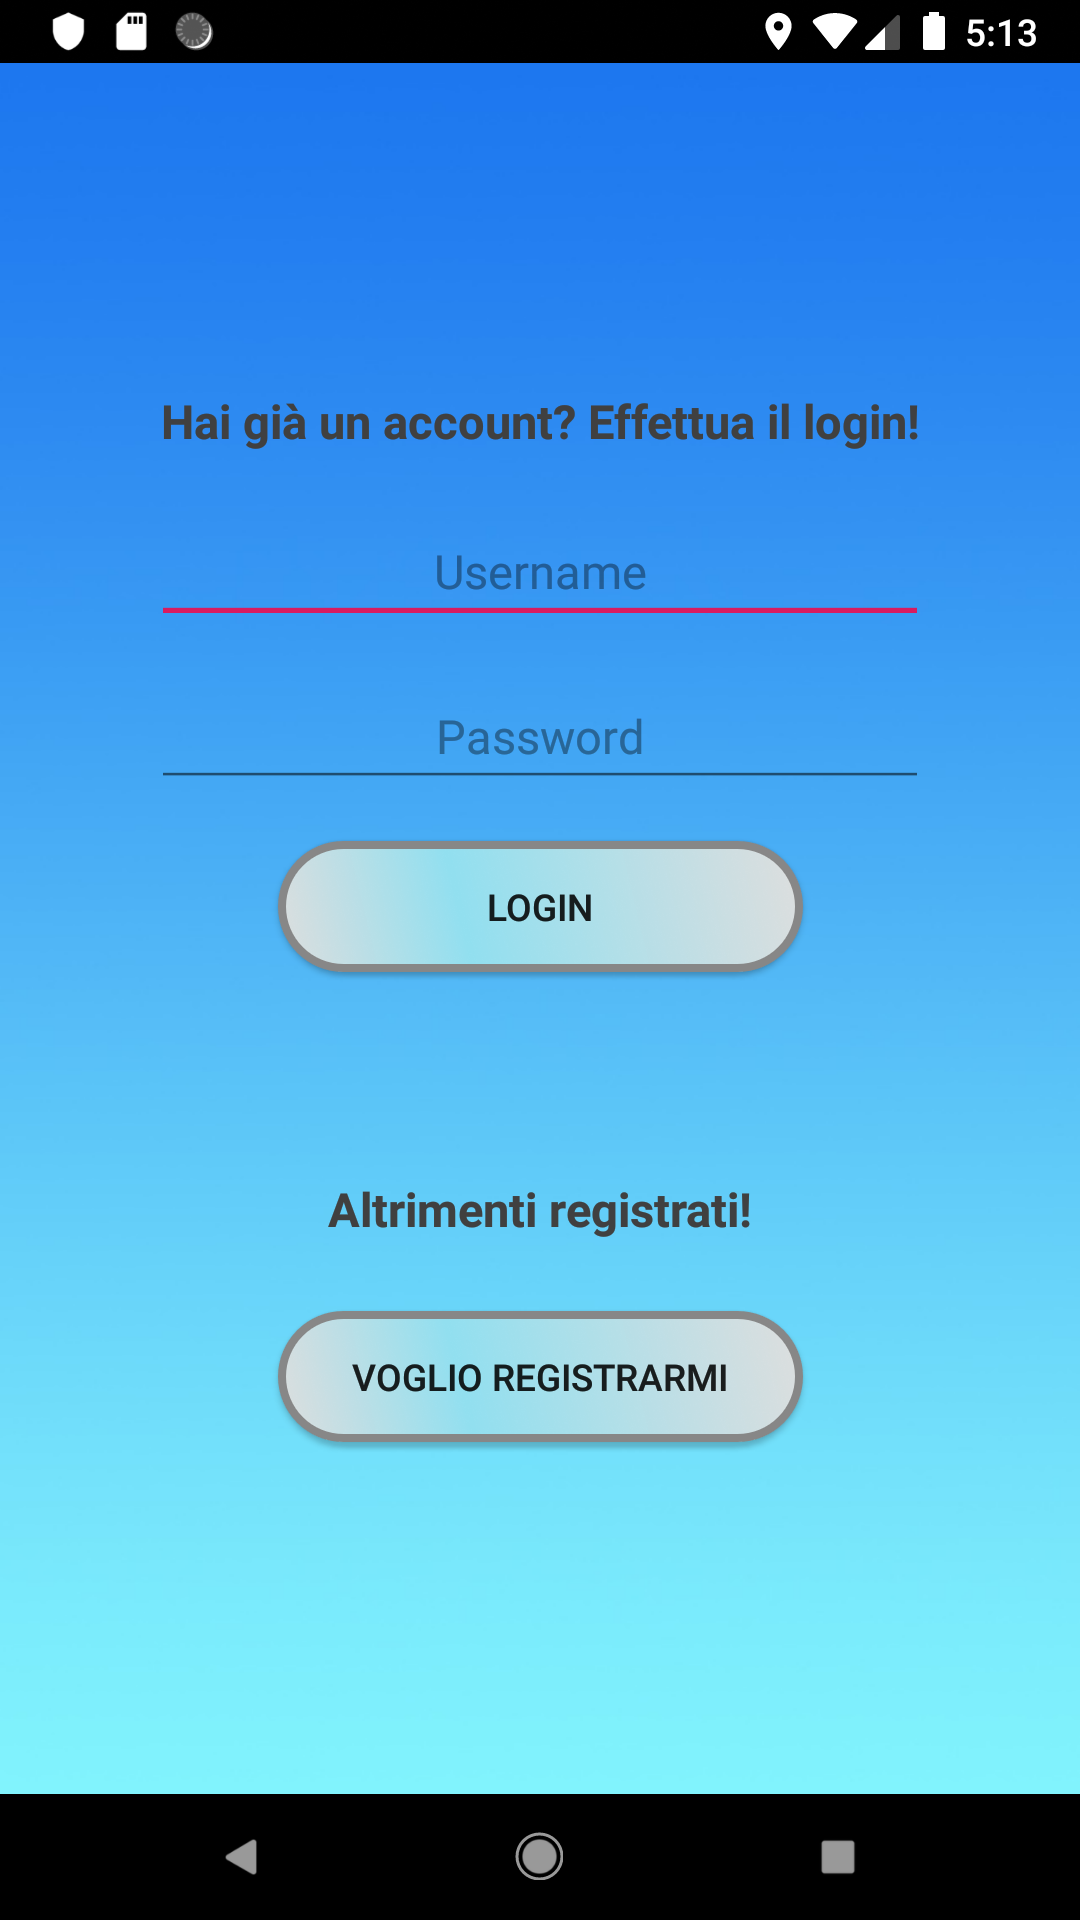
\includegraphics[width=.30\textwidth]{login}} \quad
	{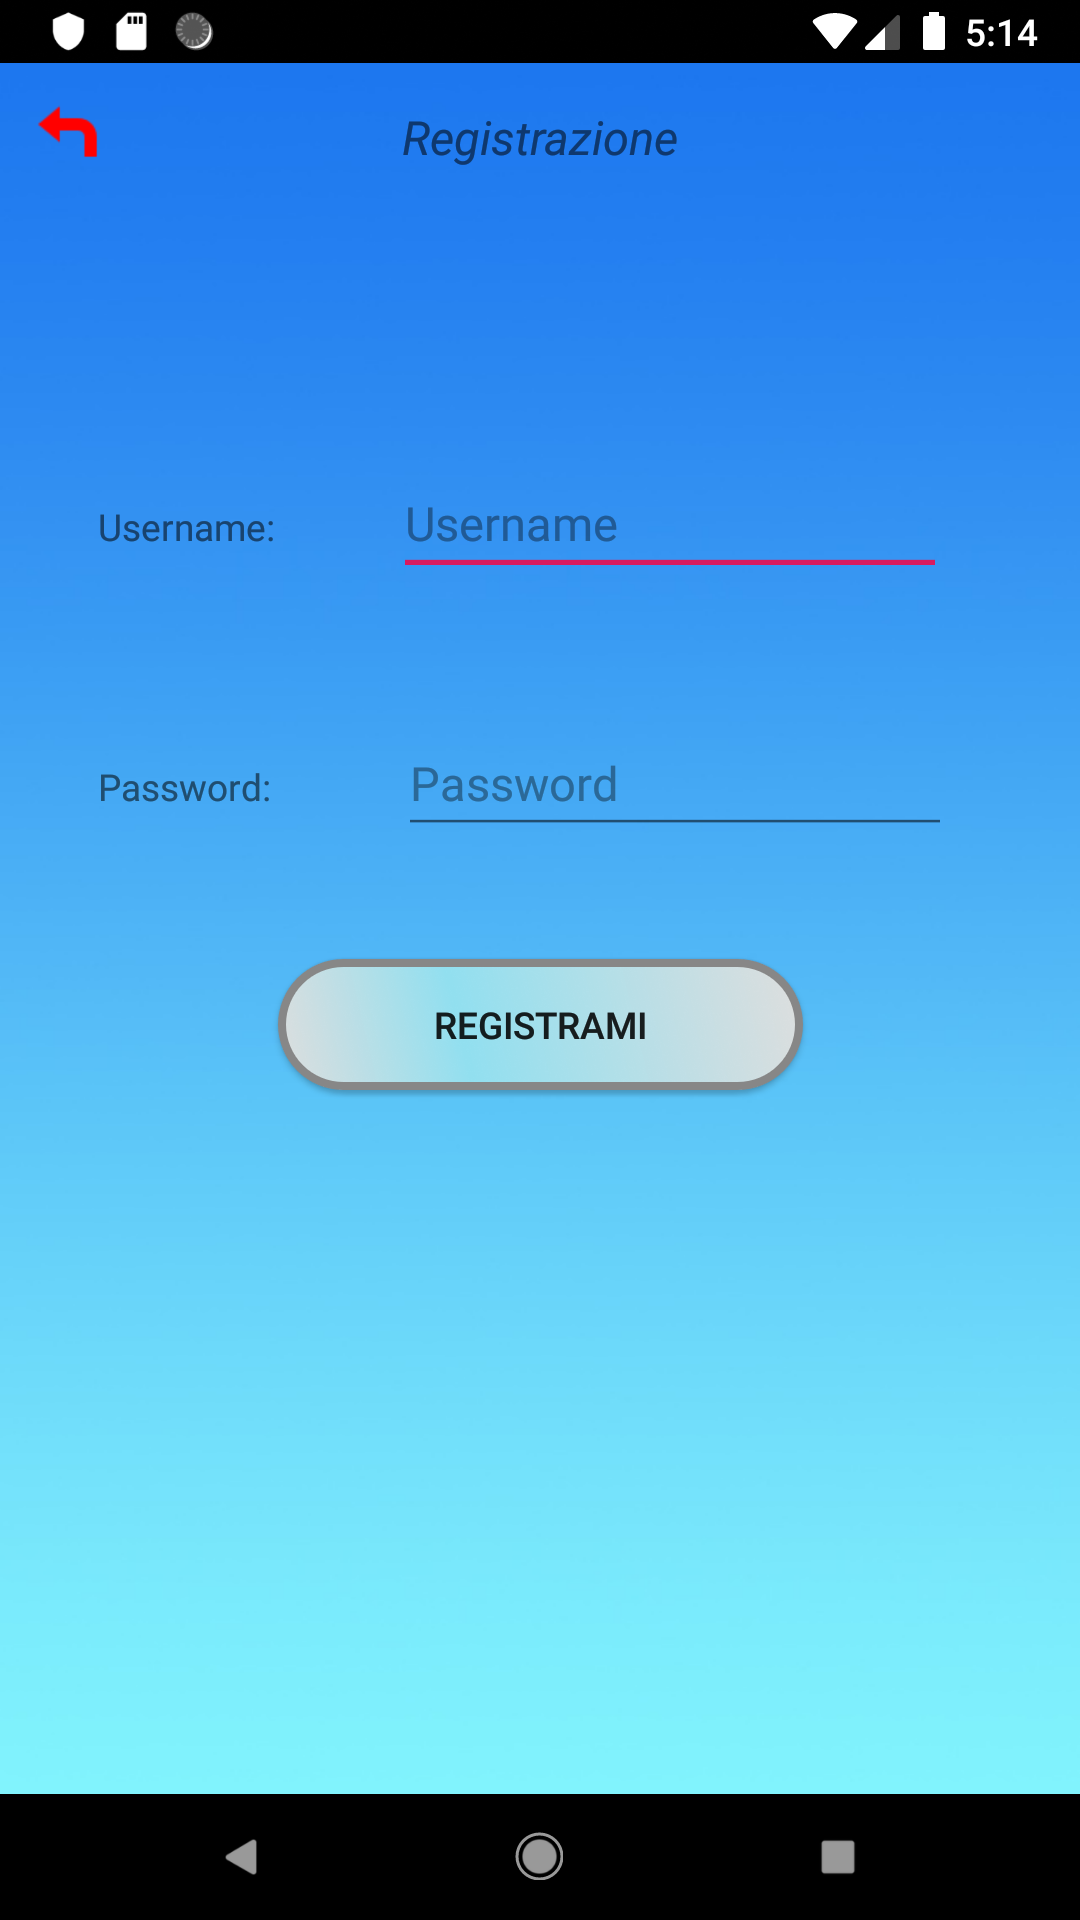
\includegraphics[width=.30\textwidth]{registrazione}} \quad
	{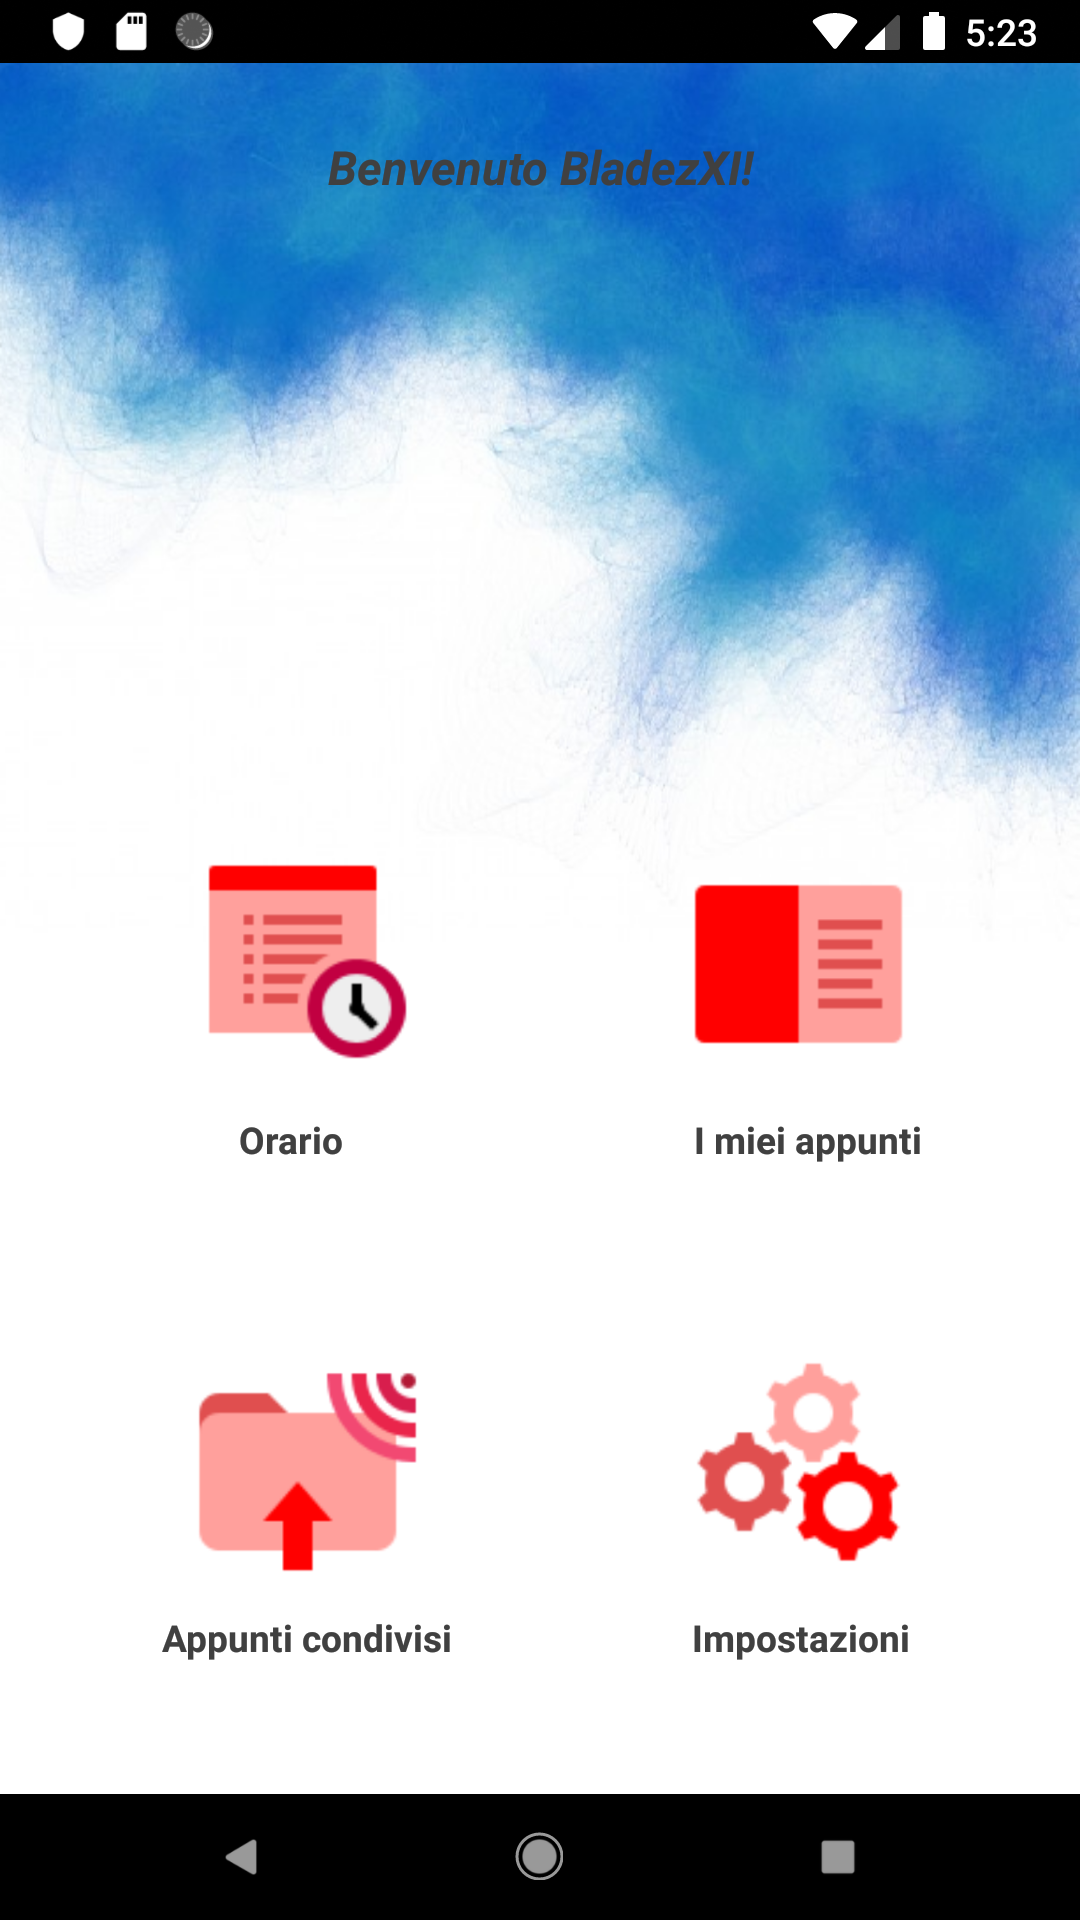
\includegraphics[width=.30\textwidth]{menu}}
	\caption{\small Schermata Login, Registrazione e Menu principale.}
\end{figure}

\newpage
\subsection{Orario}
Aperto l'orario ci si trova di fronte alla tabella relativa al giorno corrente; con la bottom navbar si può scegliere il giorno su cui andare ad agire.
Premendo nel campo \textbf{materia}, relativo all'ora di interesse si può inserire la materia in tabella, si accede, infatti, ad una lista predefinita di materie (questa può essere estesa scegliendo di inserirne una manualmente con il bottone "altro"). Scelta la materia viene visualizzata una finestra di dialogo che permette di inserire l'aula in cui si svolgerà la lezione e la durata della stessa.
\begin{figure}[!h]
	\centering
	{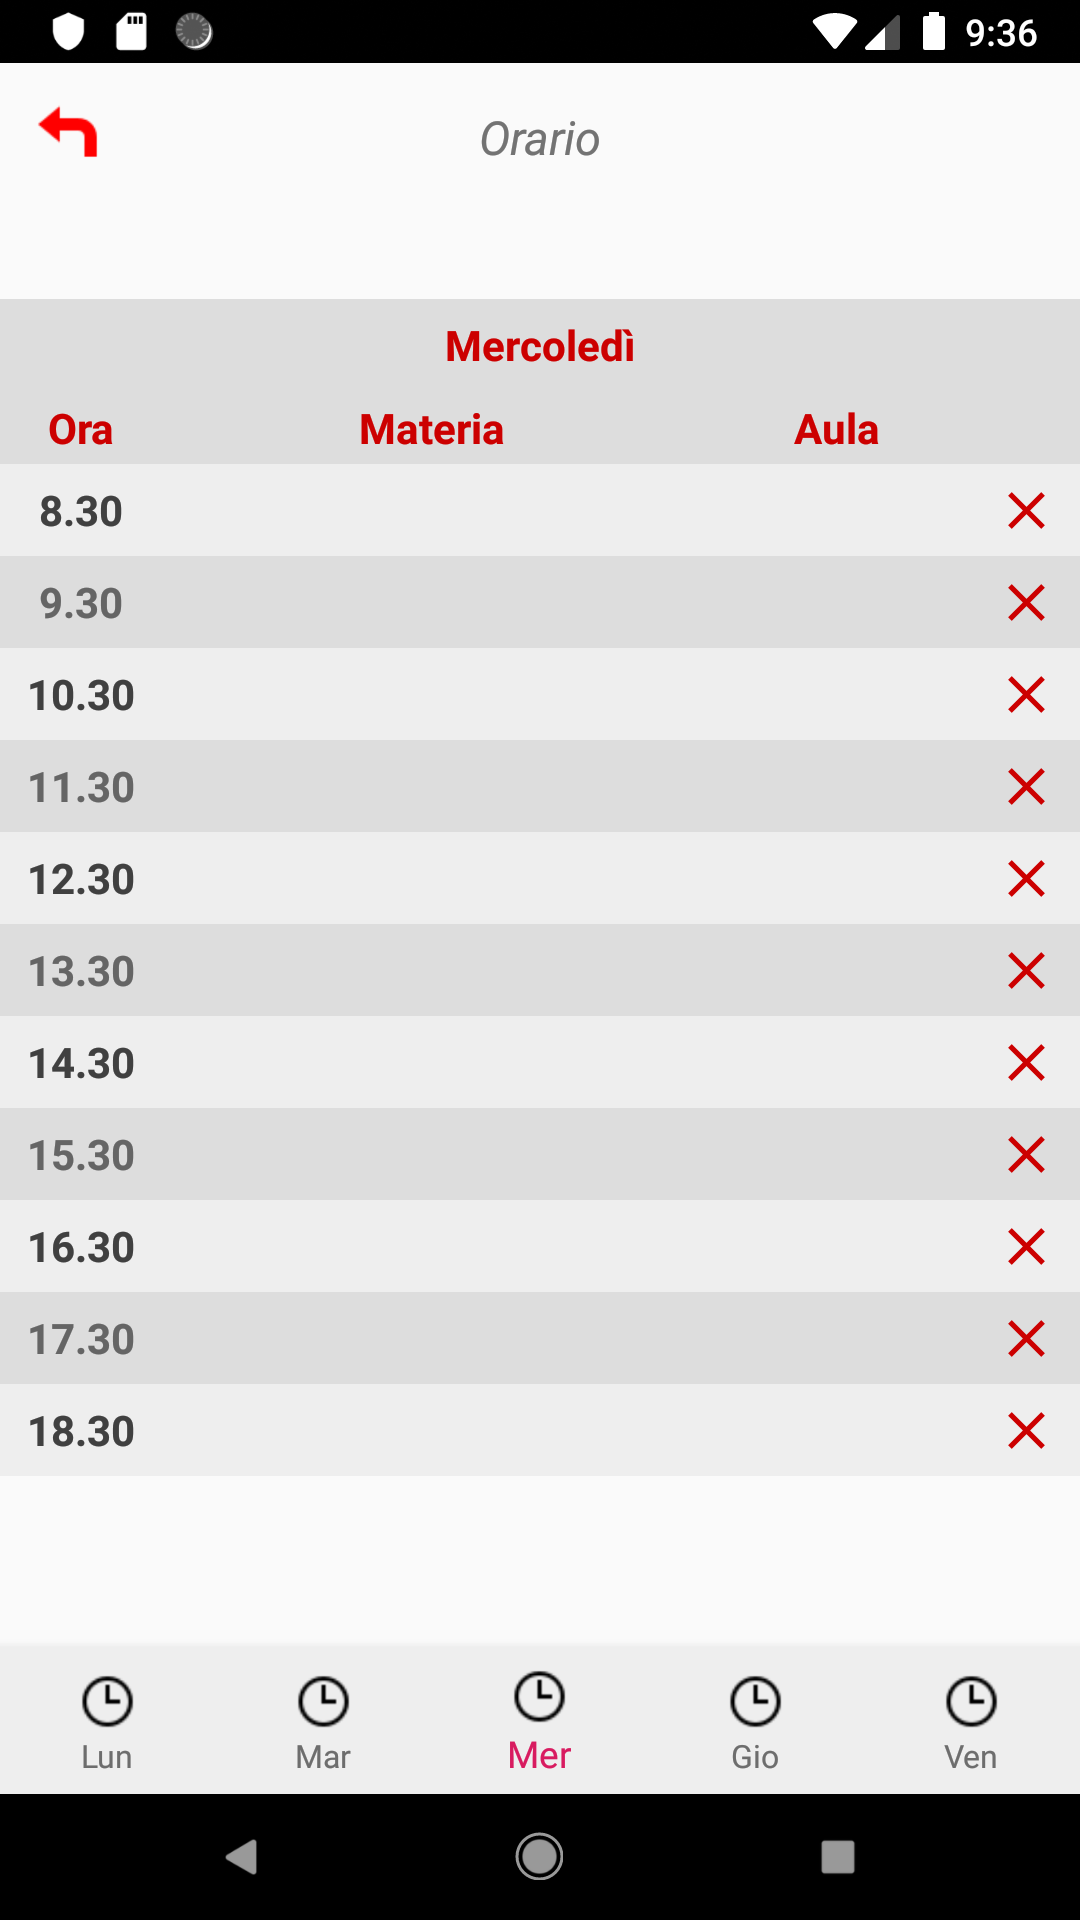
\includegraphics[width=.30\textwidth]{orario}} \quad
	{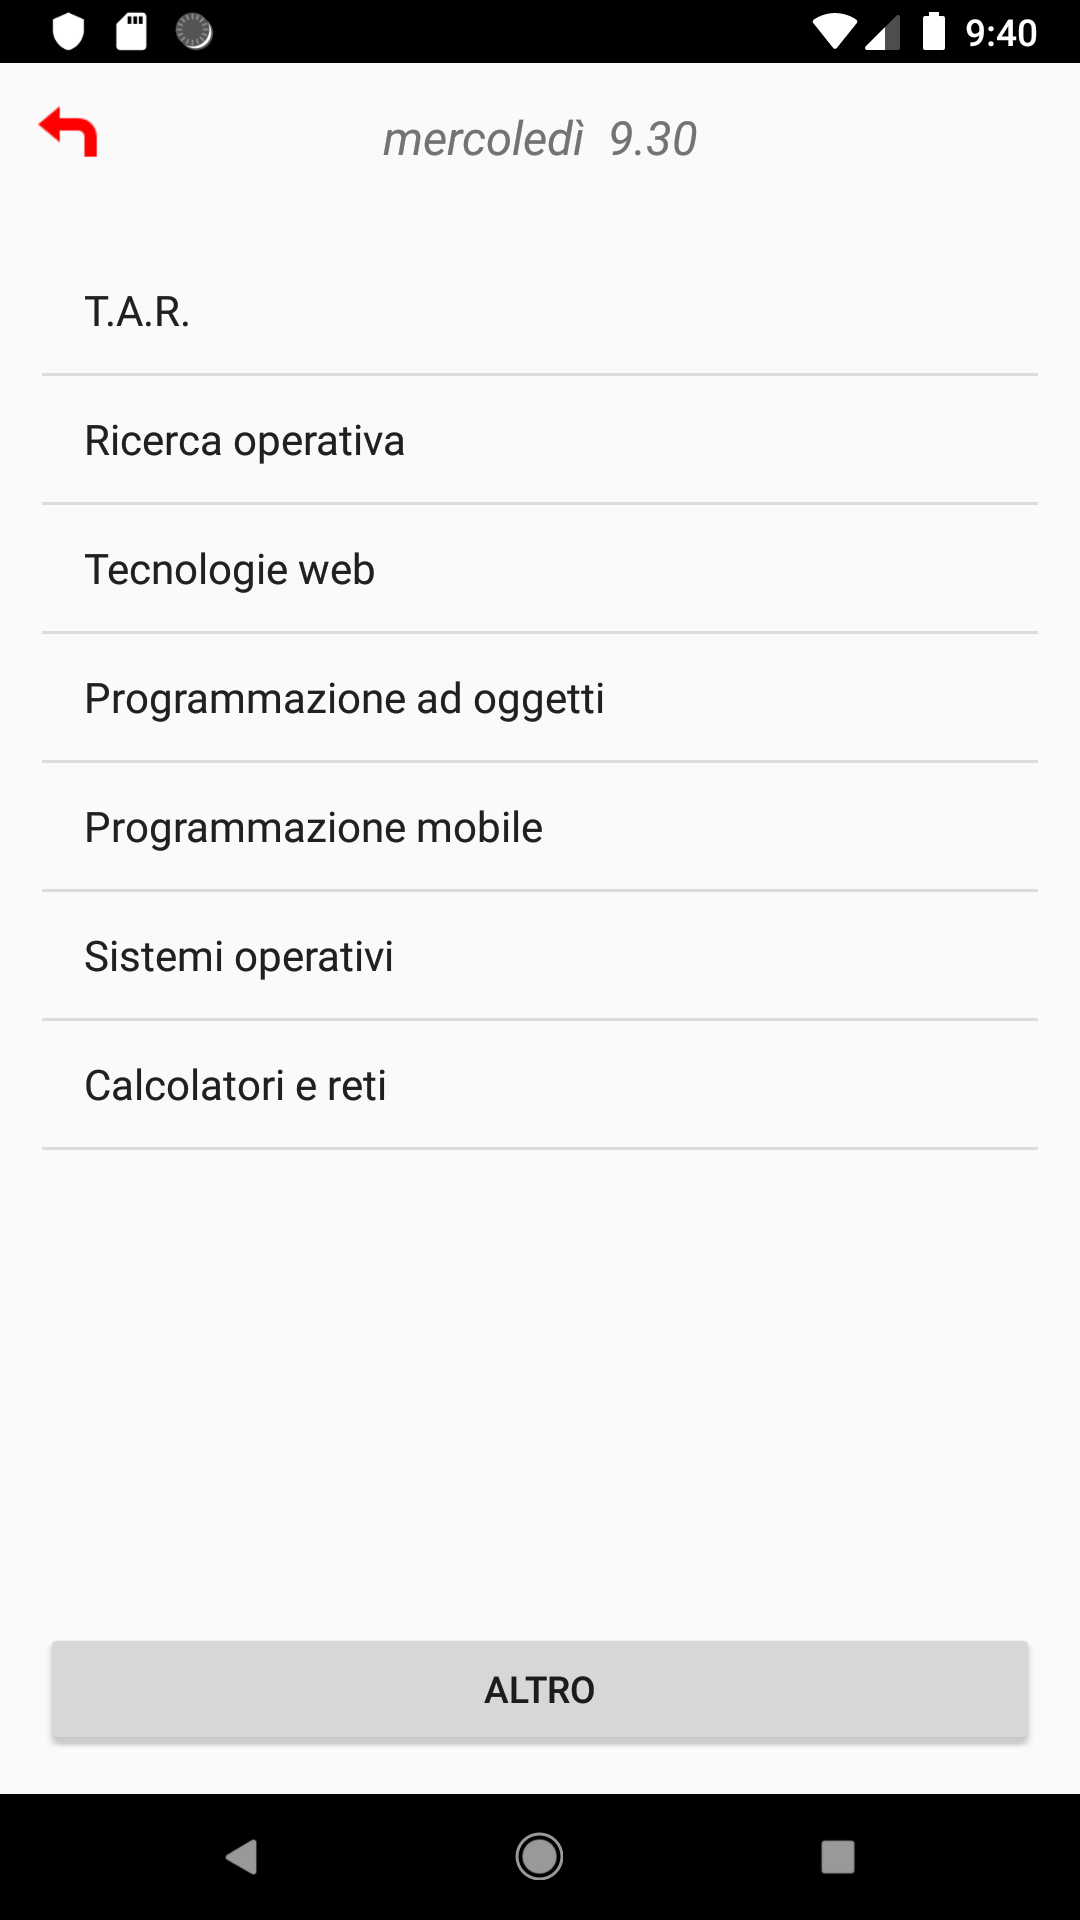
\includegraphics[width=.30\textwidth]{orario_scelta_materia}}\quad
	{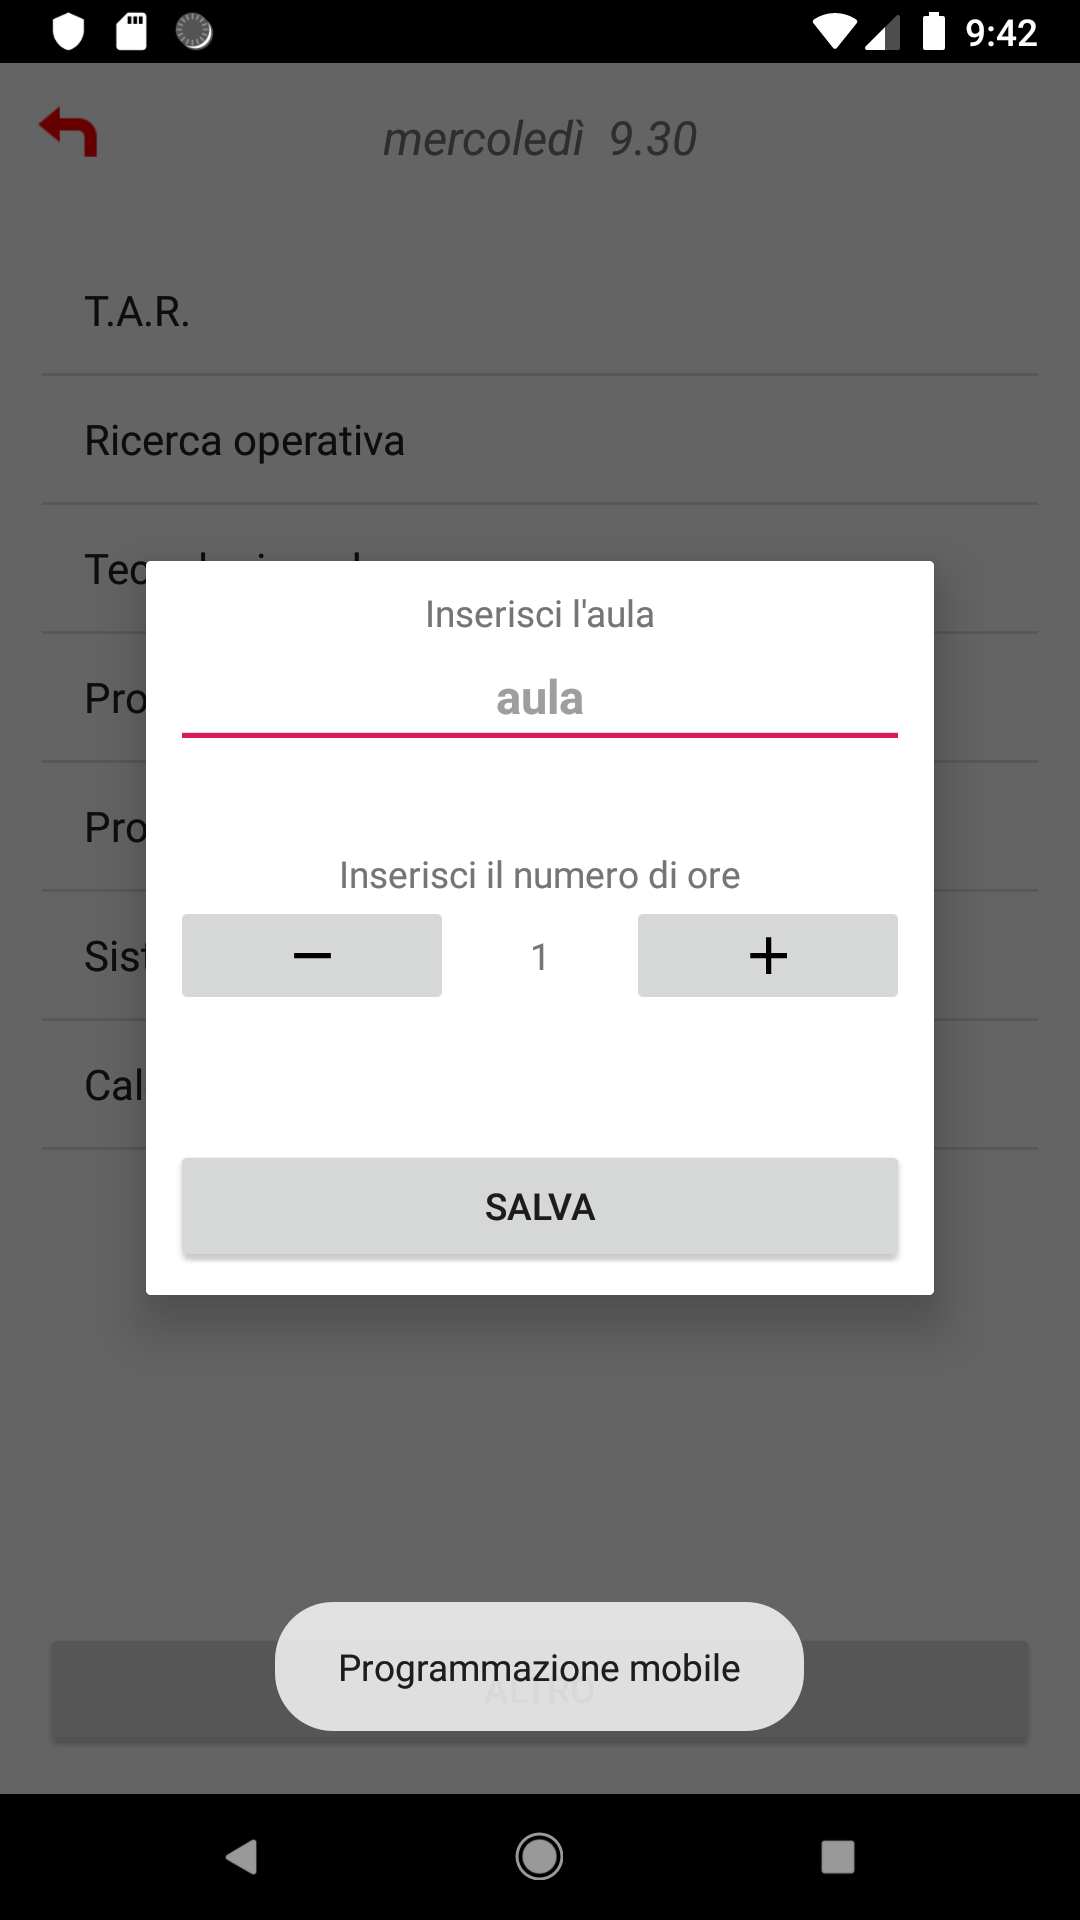
\includegraphics[width=.30\textwidth]{orario_inserimento}}
	\caption{\small Orario.}
\end{figure}

Salvata la materia nell'orario questa viene salvata nel database e inserita in una lista nella sezione \textbf{i miei appunti}.

\subsection{I miei appunti}
In questa sezione abbiamo accesso alla lista di tutte le materie salvate nel database. Abbiamo la possibilità di aggiungerne altre a piacimento o eliminarle inserendo il nome esatto della materia.

\begin{figure}[!h]
	\centering
	{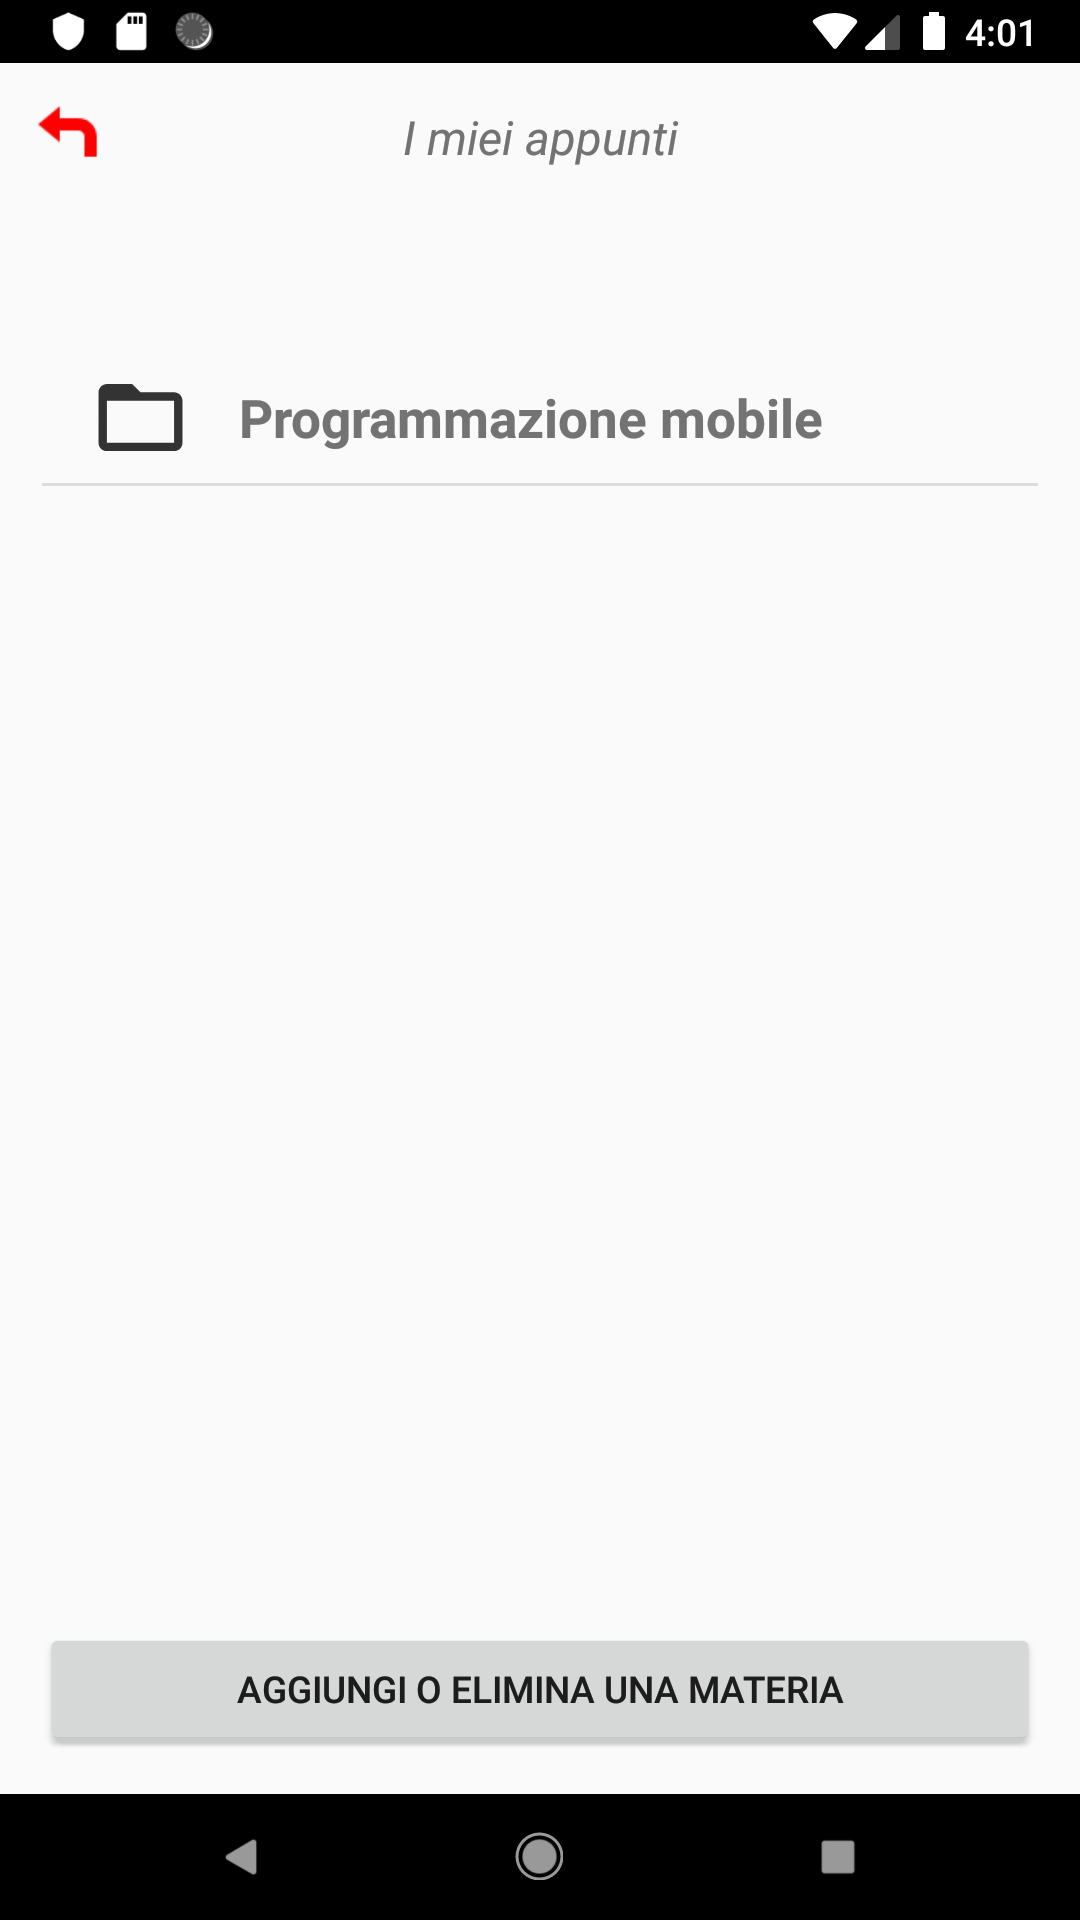
\includegraphics[width=.30\textwidth]{miei_appunti_lista_materie}} \quad
	{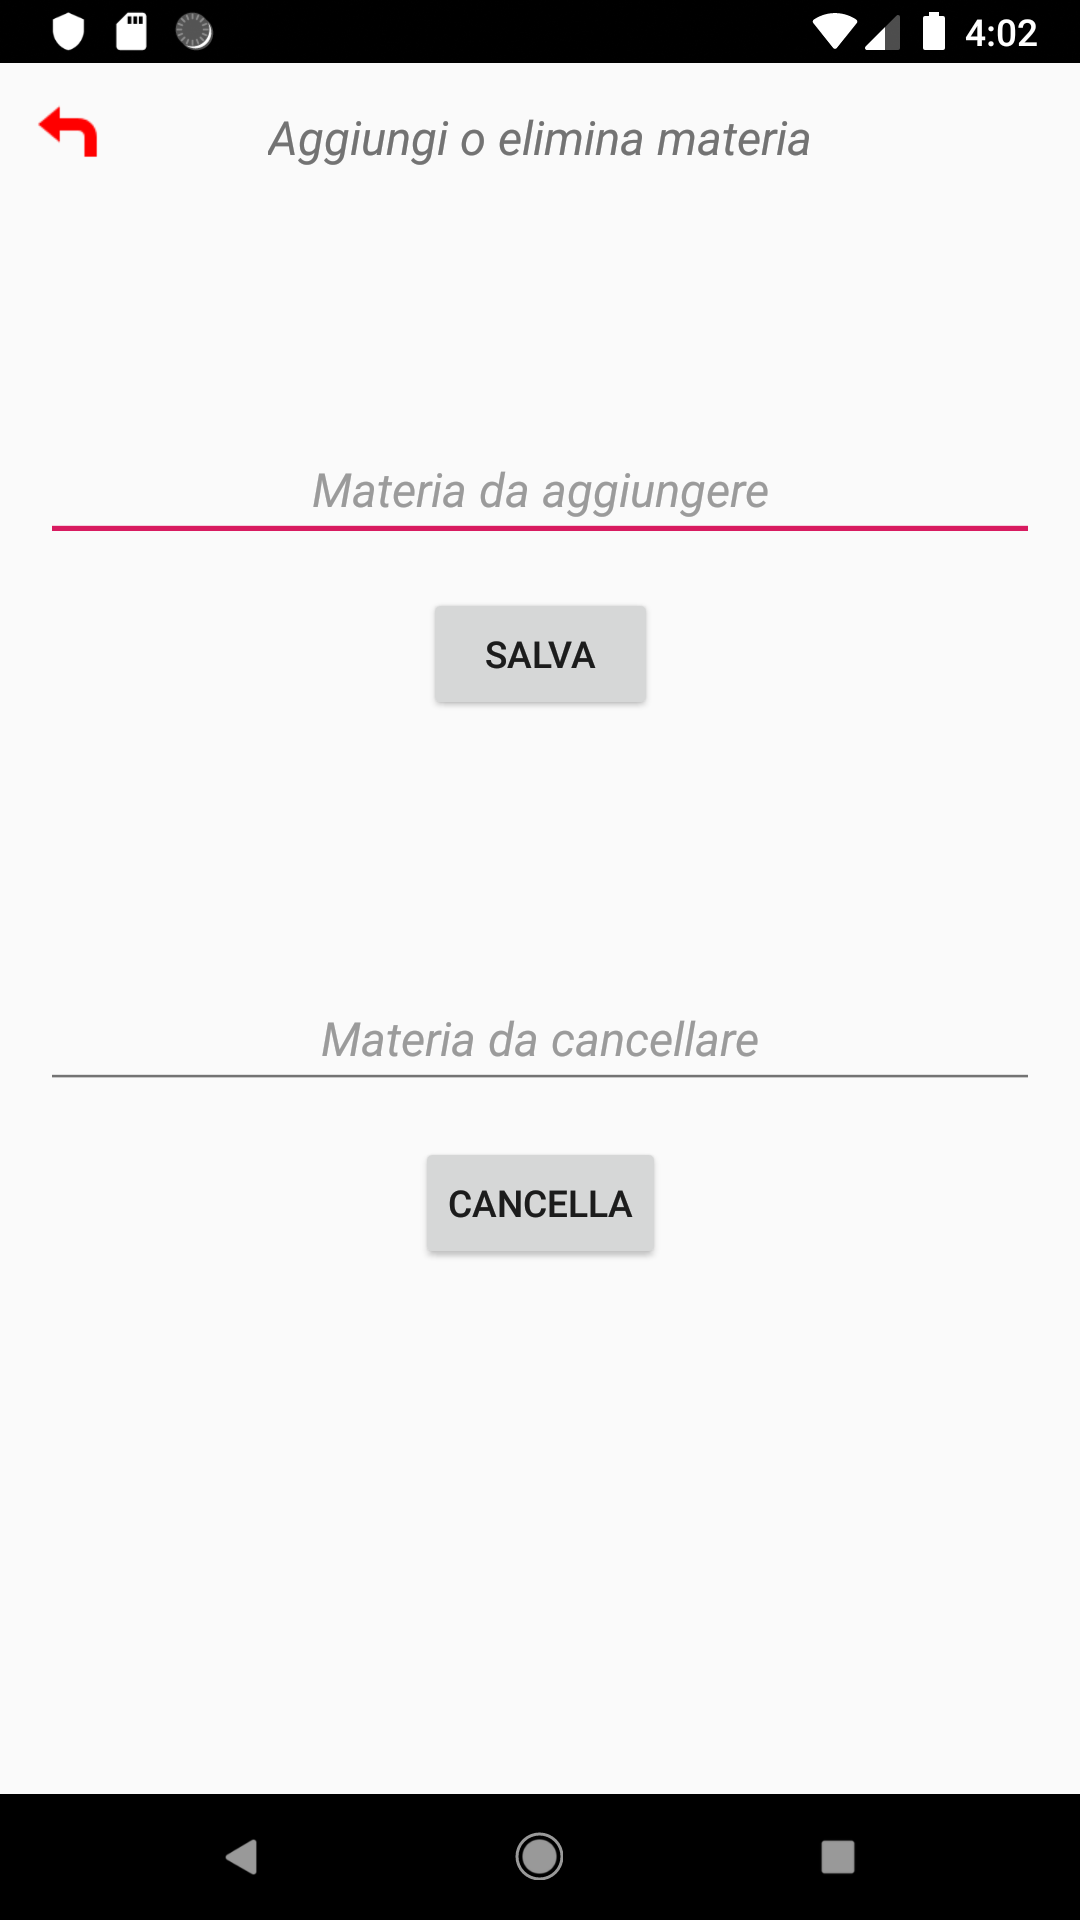
\includegraphics[width=.30\textwidth]{miei_appunti_aggiungi_materia}} \quad
	{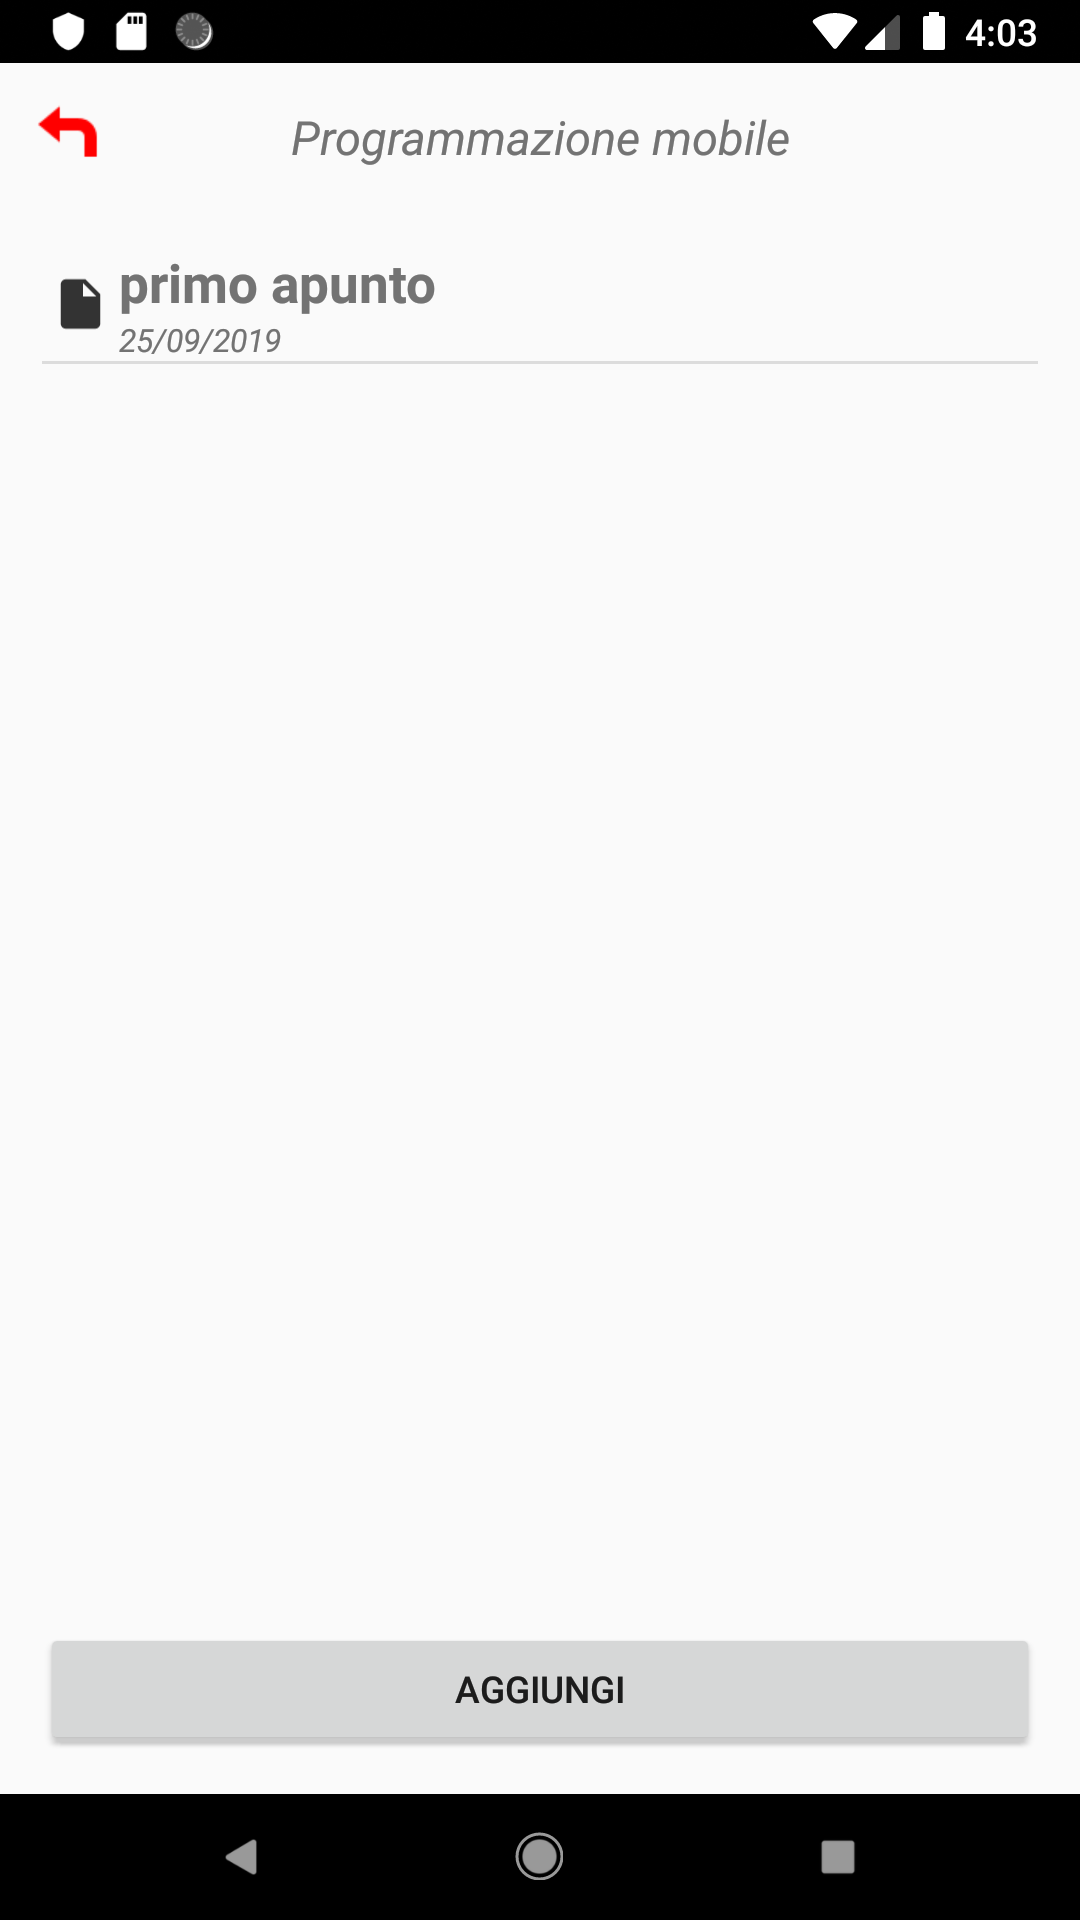
\includegraphics[width=.30\textwidth]{miei_appunti_lista_appunti}}
	\caption{\small Scegli aggiungi o elimina una materia e scegli un appunto.}
\end{figure}

Scelta la materia accediamo ad una seconda lista contenente tutti gli appunti relativi ad essa; ogni elemento della lsita contiene titolo e data relativi ad ogni appunto.
Da questa lista possiamo accedere e visualizzare l'annotazione vera e propria.

Gli appunti possono essere aggiunti con il bottone \textbf{"aggiungi"}, qui inseriremo titolo data e annotazione che vogliamo salvare; da questa schermata, inserendo la spunta nel campo \textbf{"Condividi"}, possono essere condivisi direttamente gli appunti con gli altri utenti.

Per eliminare un appunto basta tenere premuto l'elemento da eliminare, verrà attivata una finestra di dialogo da cui è possibile confermare la cancellazione.

\begin{figure}[!h]
	\centering
	{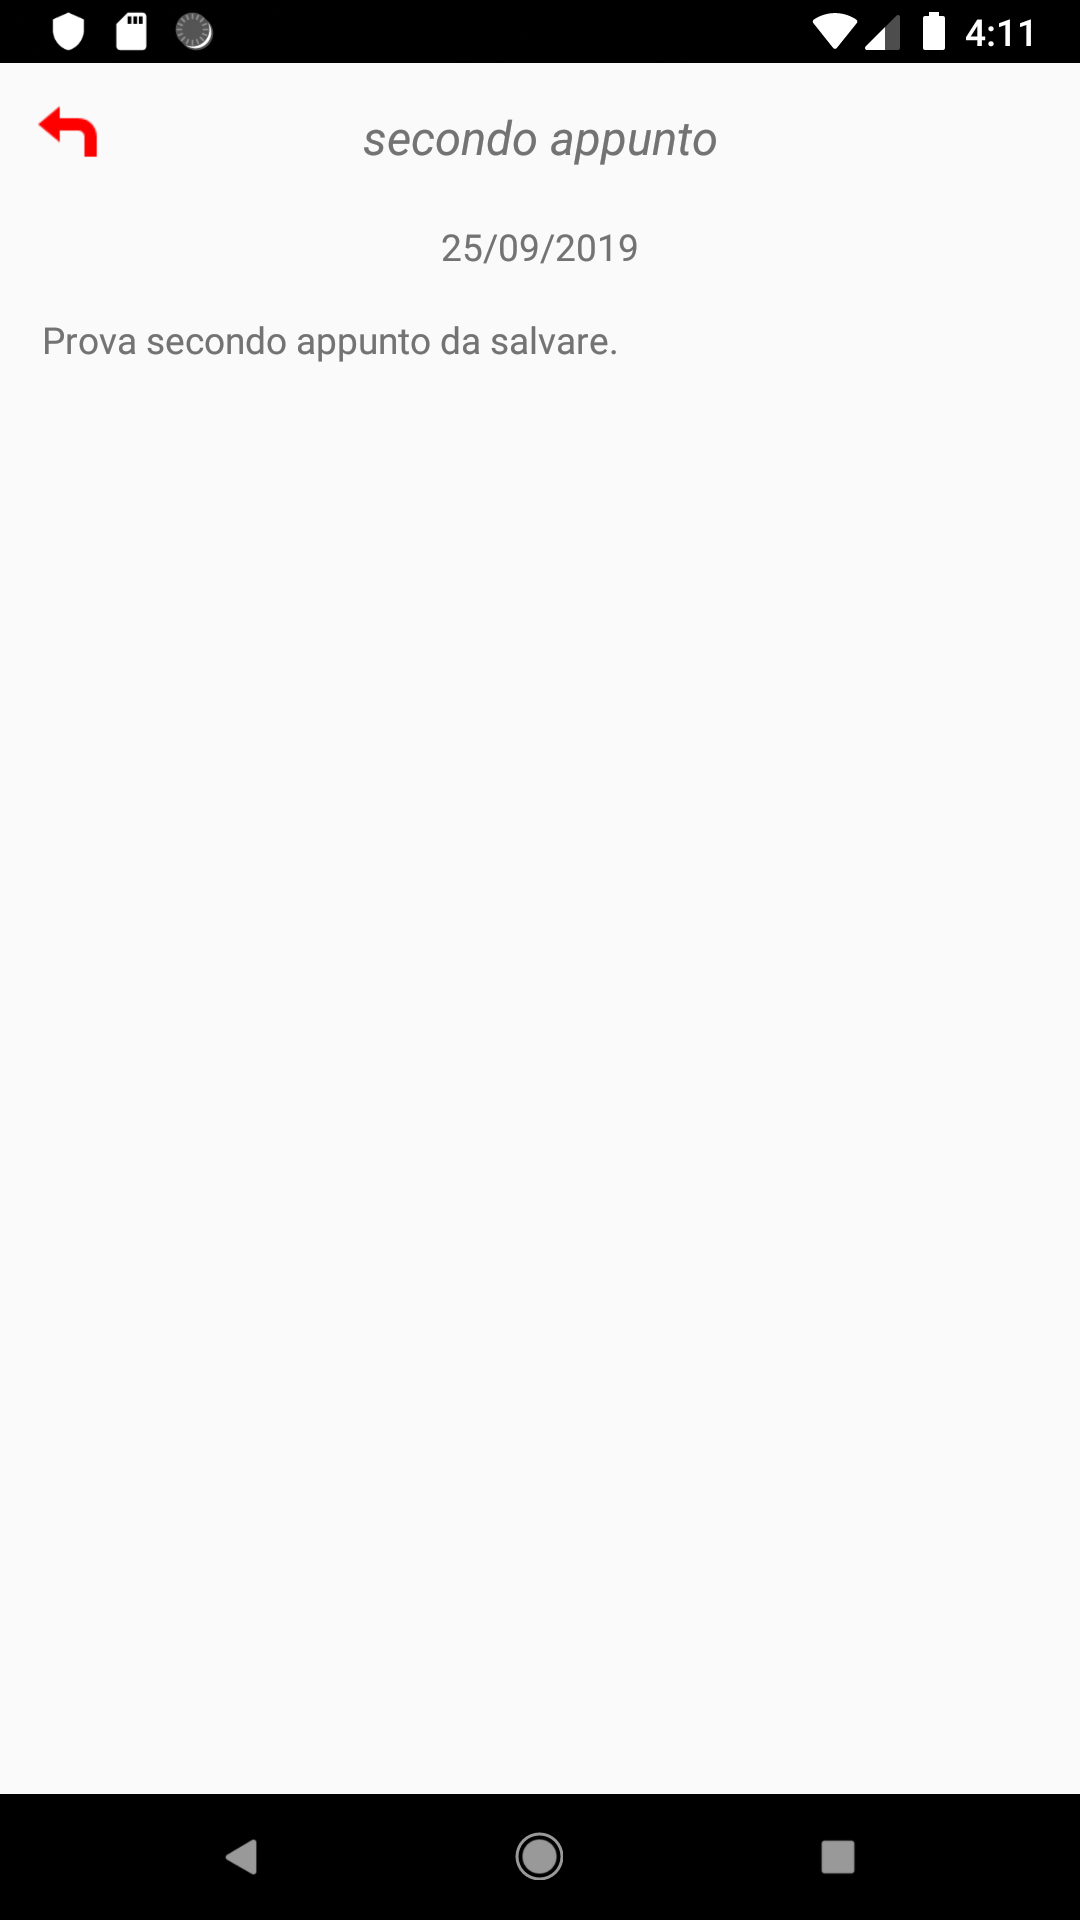
\includegraphics[width=.30\textwidth]{miei_appunti_vedi_appunto}} \quad
	{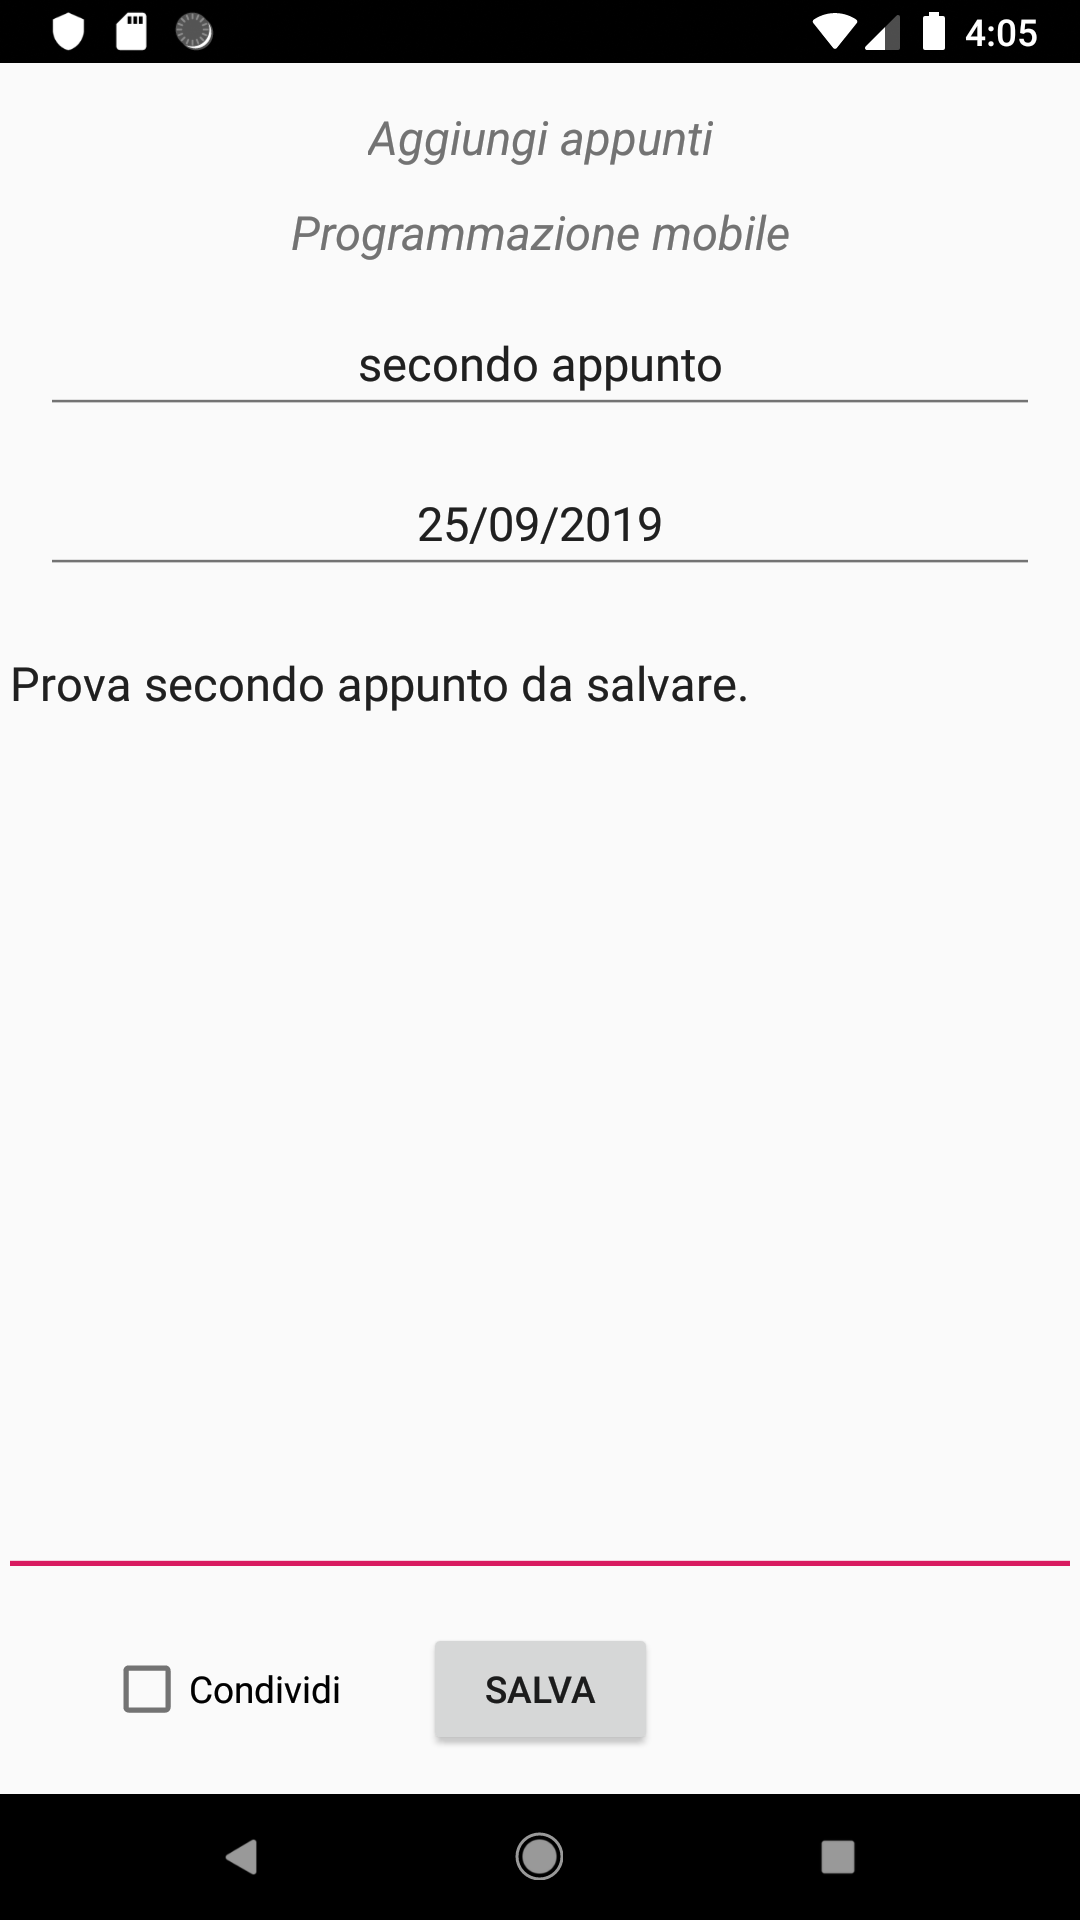
\includegraphics[width=.30\textwidth]{miei_appunti_aggiungi_appunto}} \quad
	{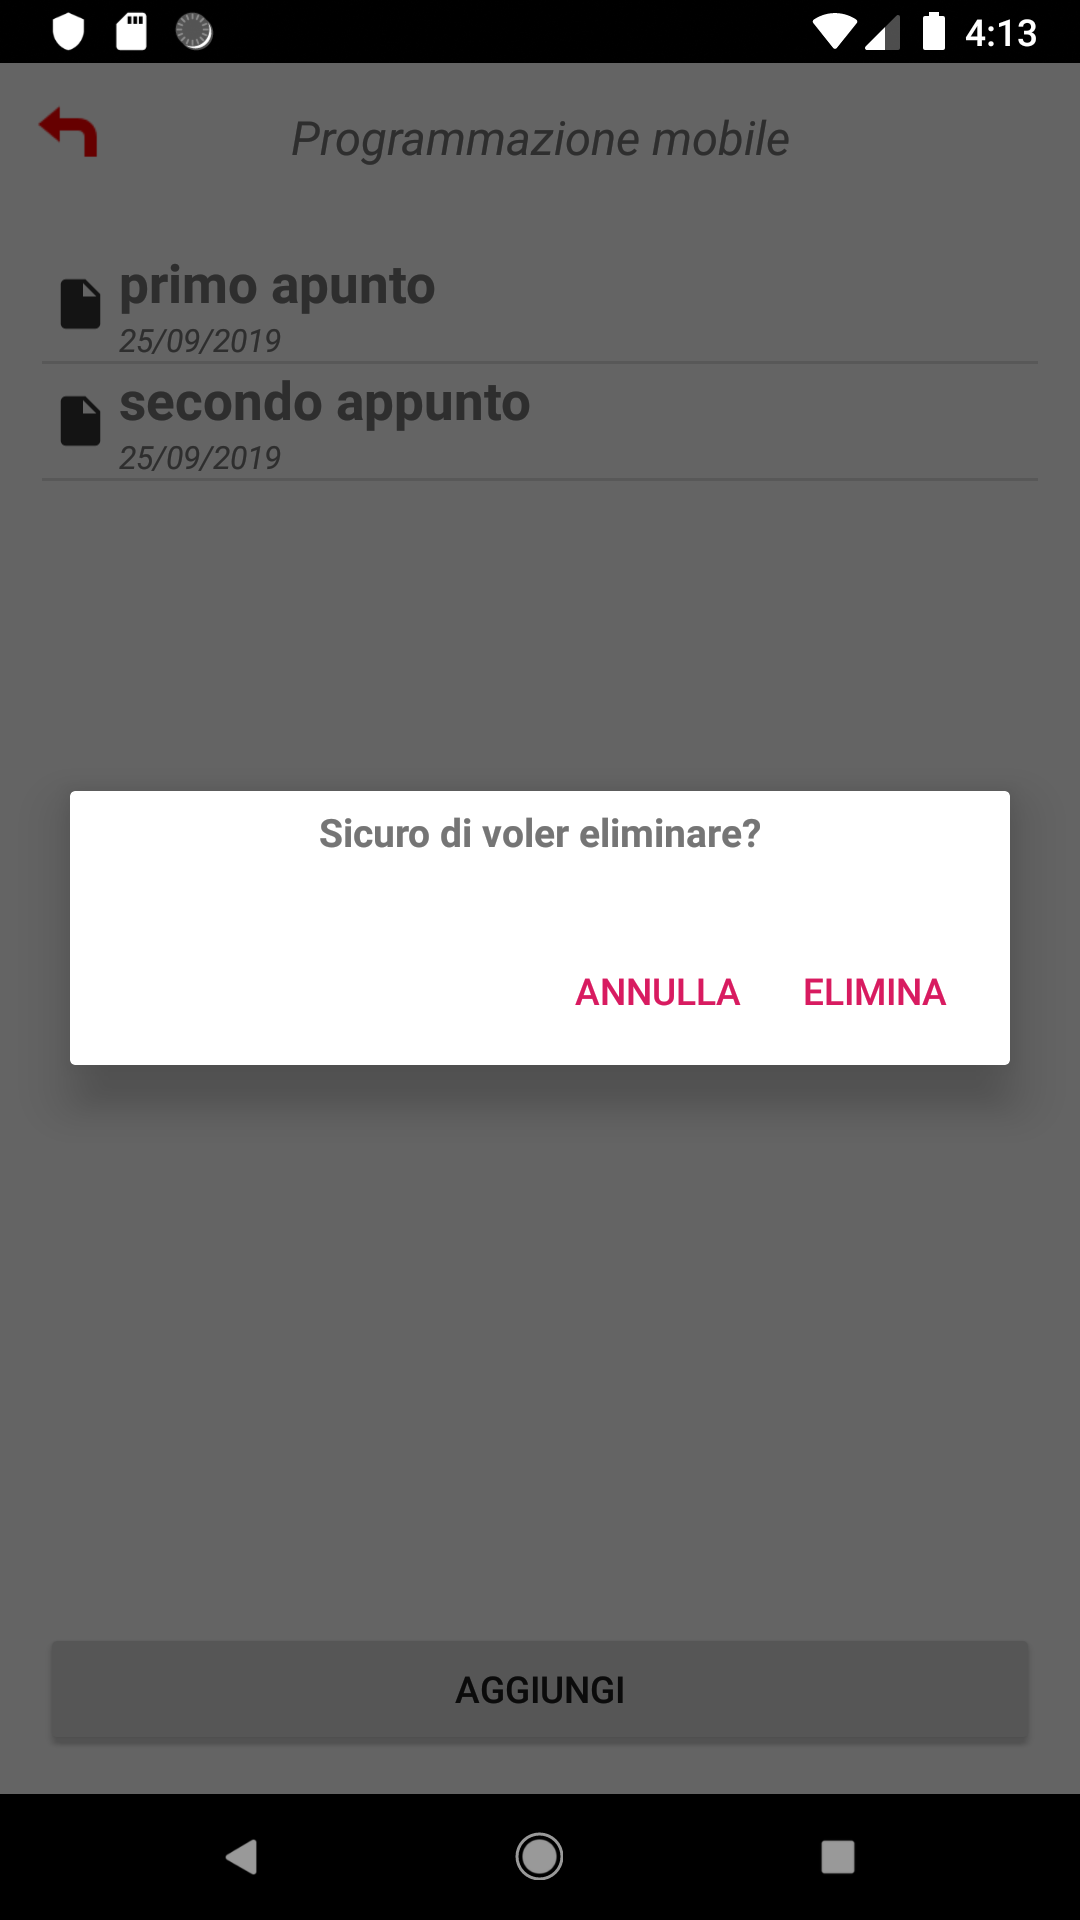
\includegraphics[width=.30\textwidth]{miei_appunti_elimina_appunto}}
	\caption{\small Visualizza, aggiungi o elimina un appunto.}
\end{figure}

\subsection{Appunti condivisi}
Nella sezione appunti condivisi possiamo scegliere una delle materie predefinite in lista per visualizzare gli appunti che sono stati condivisi ed eventualmente visualizzarli o scaricarli.

\begin{figure}[!h]
	\centering
	{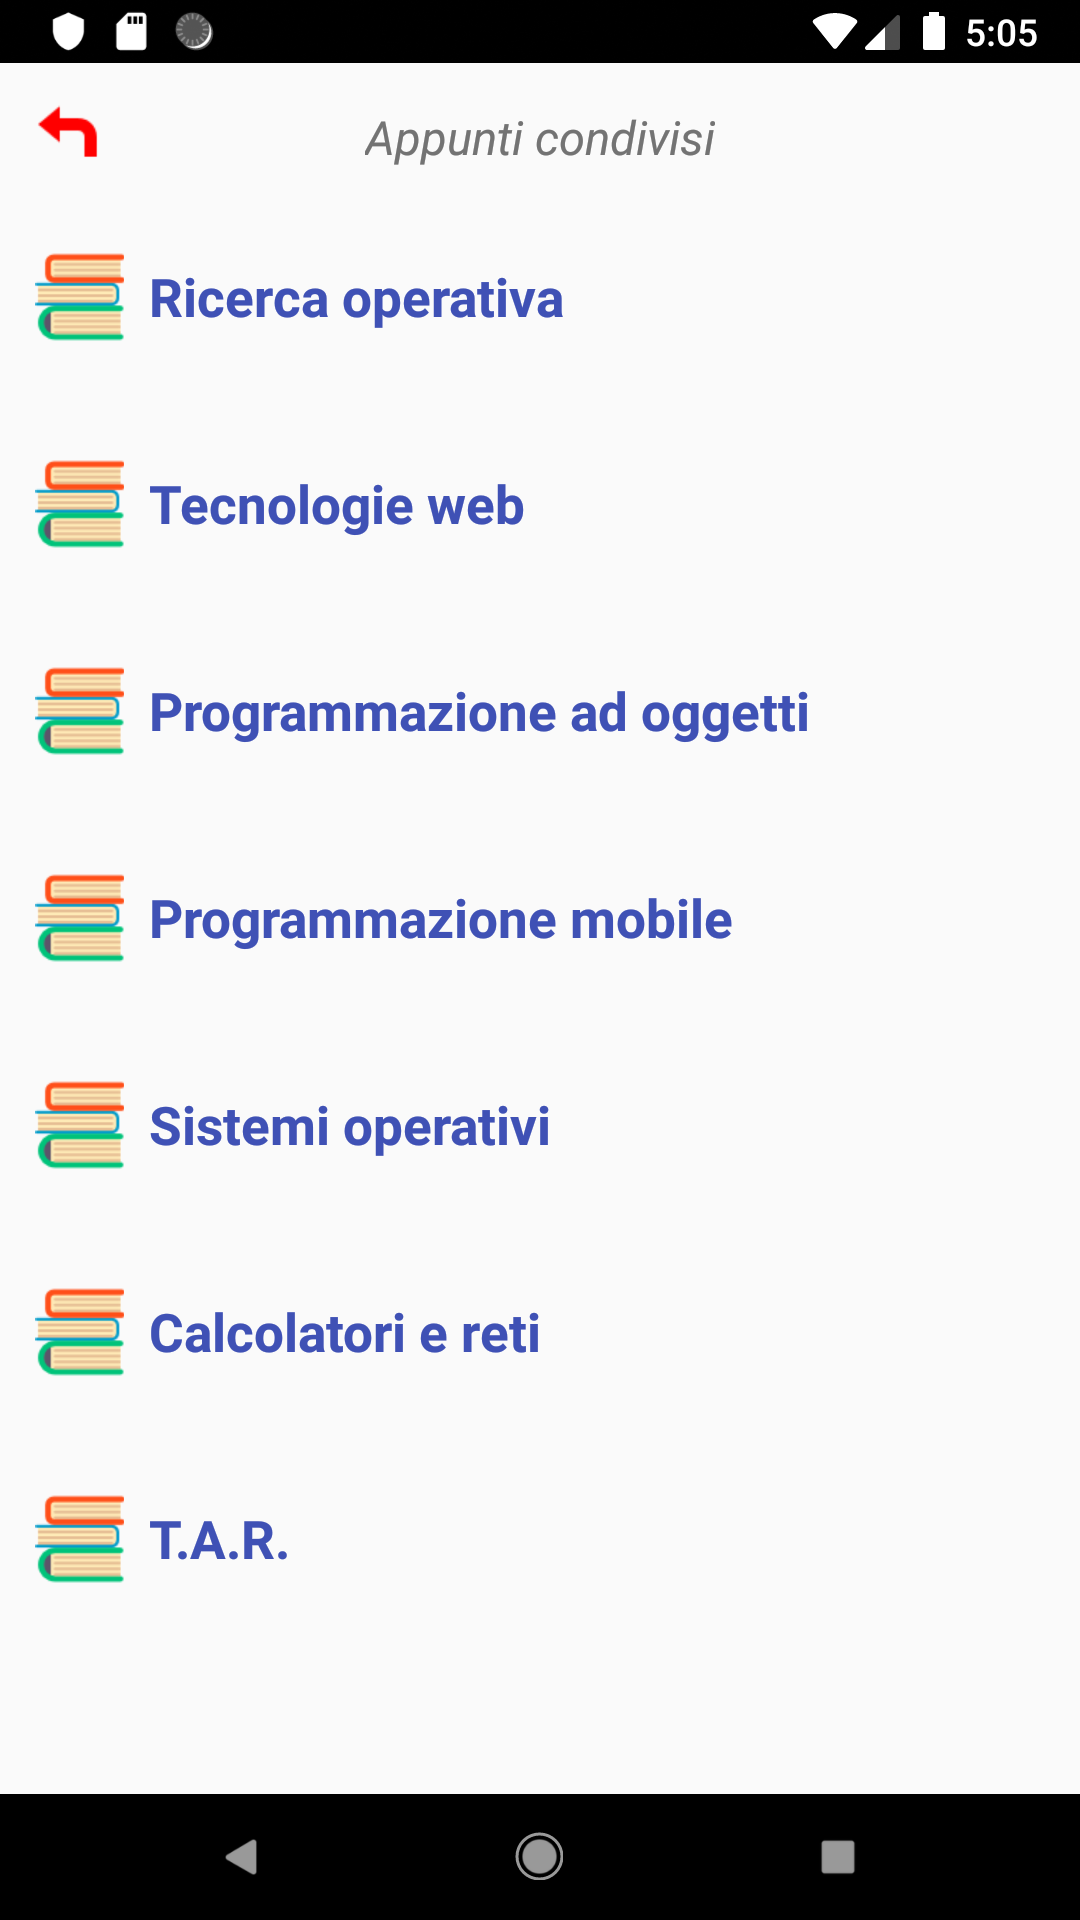
\includegraphics[width=.30\textwidth]{appunti_condivisi_lista_materie}} \quad
	{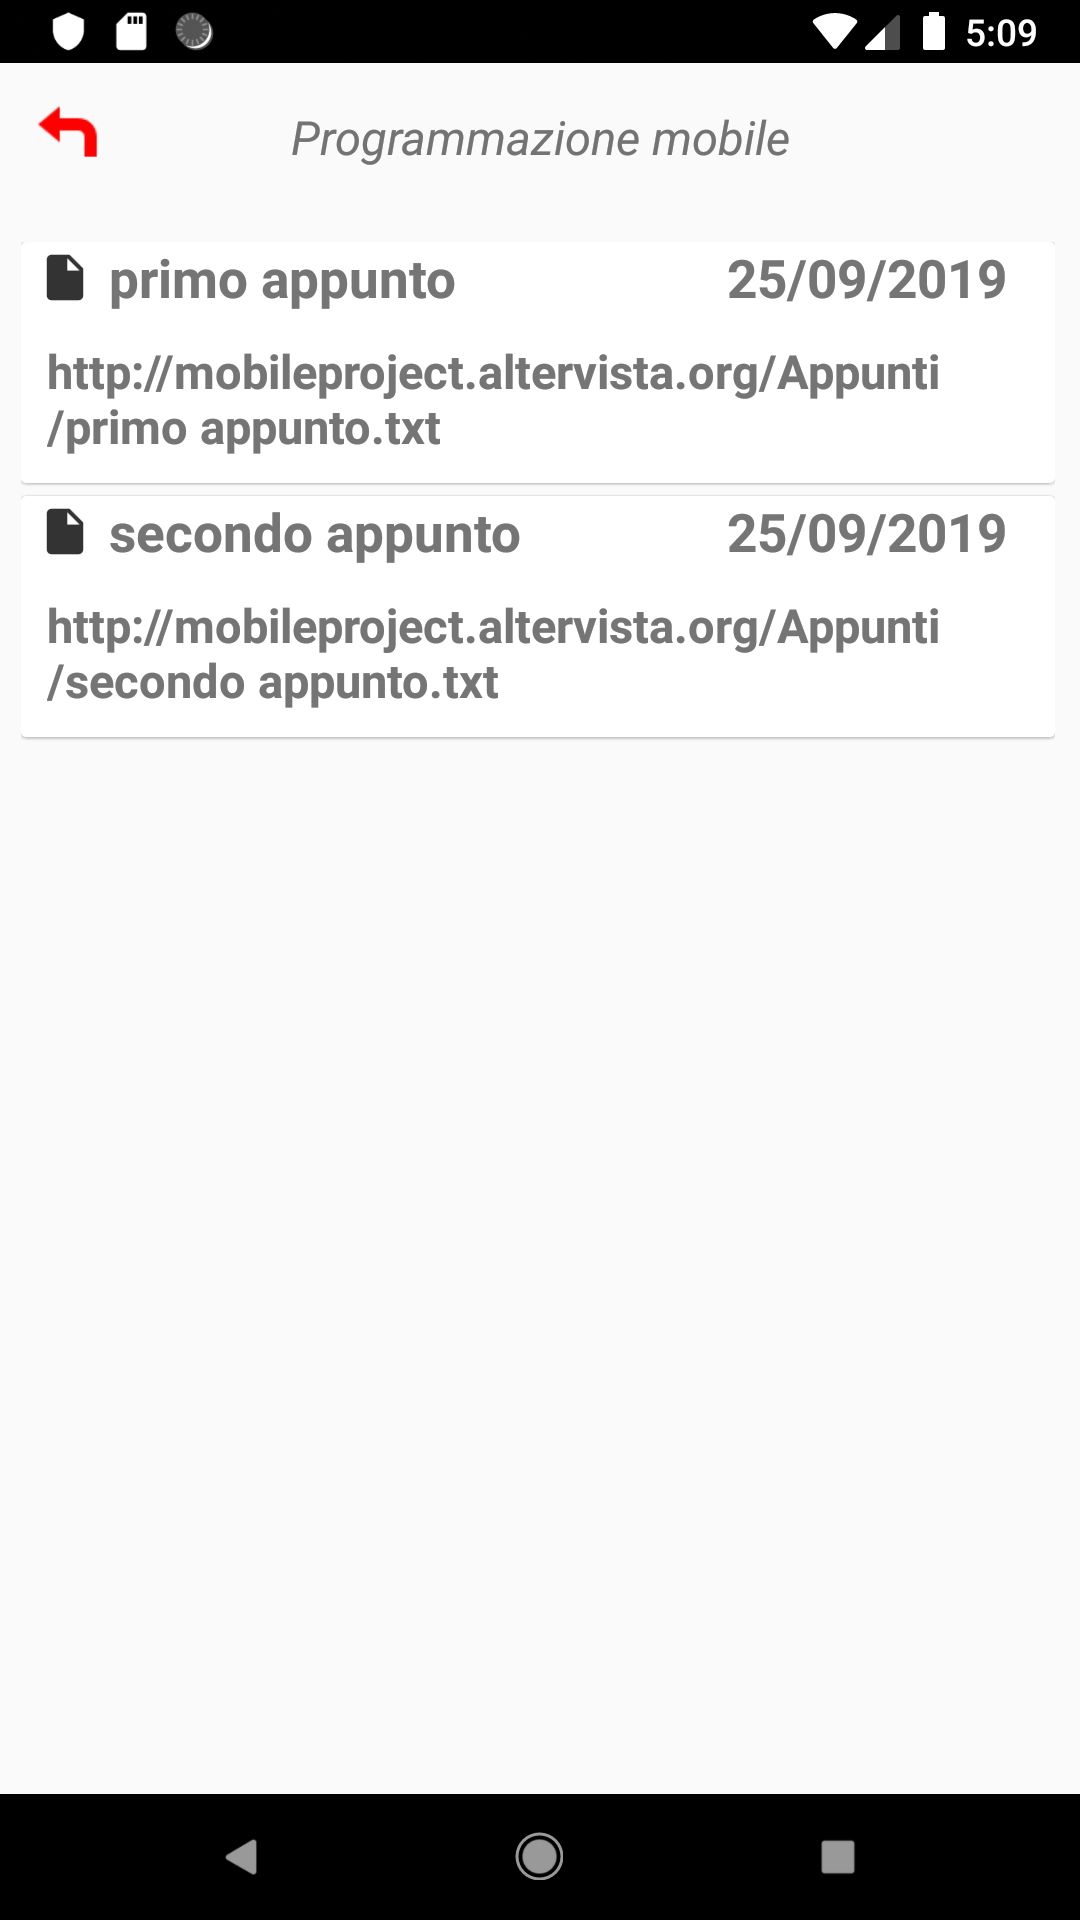
\includegraphics[width=.30\textwidth]{appunti_condivisi_lista_appunti}} \quad
	{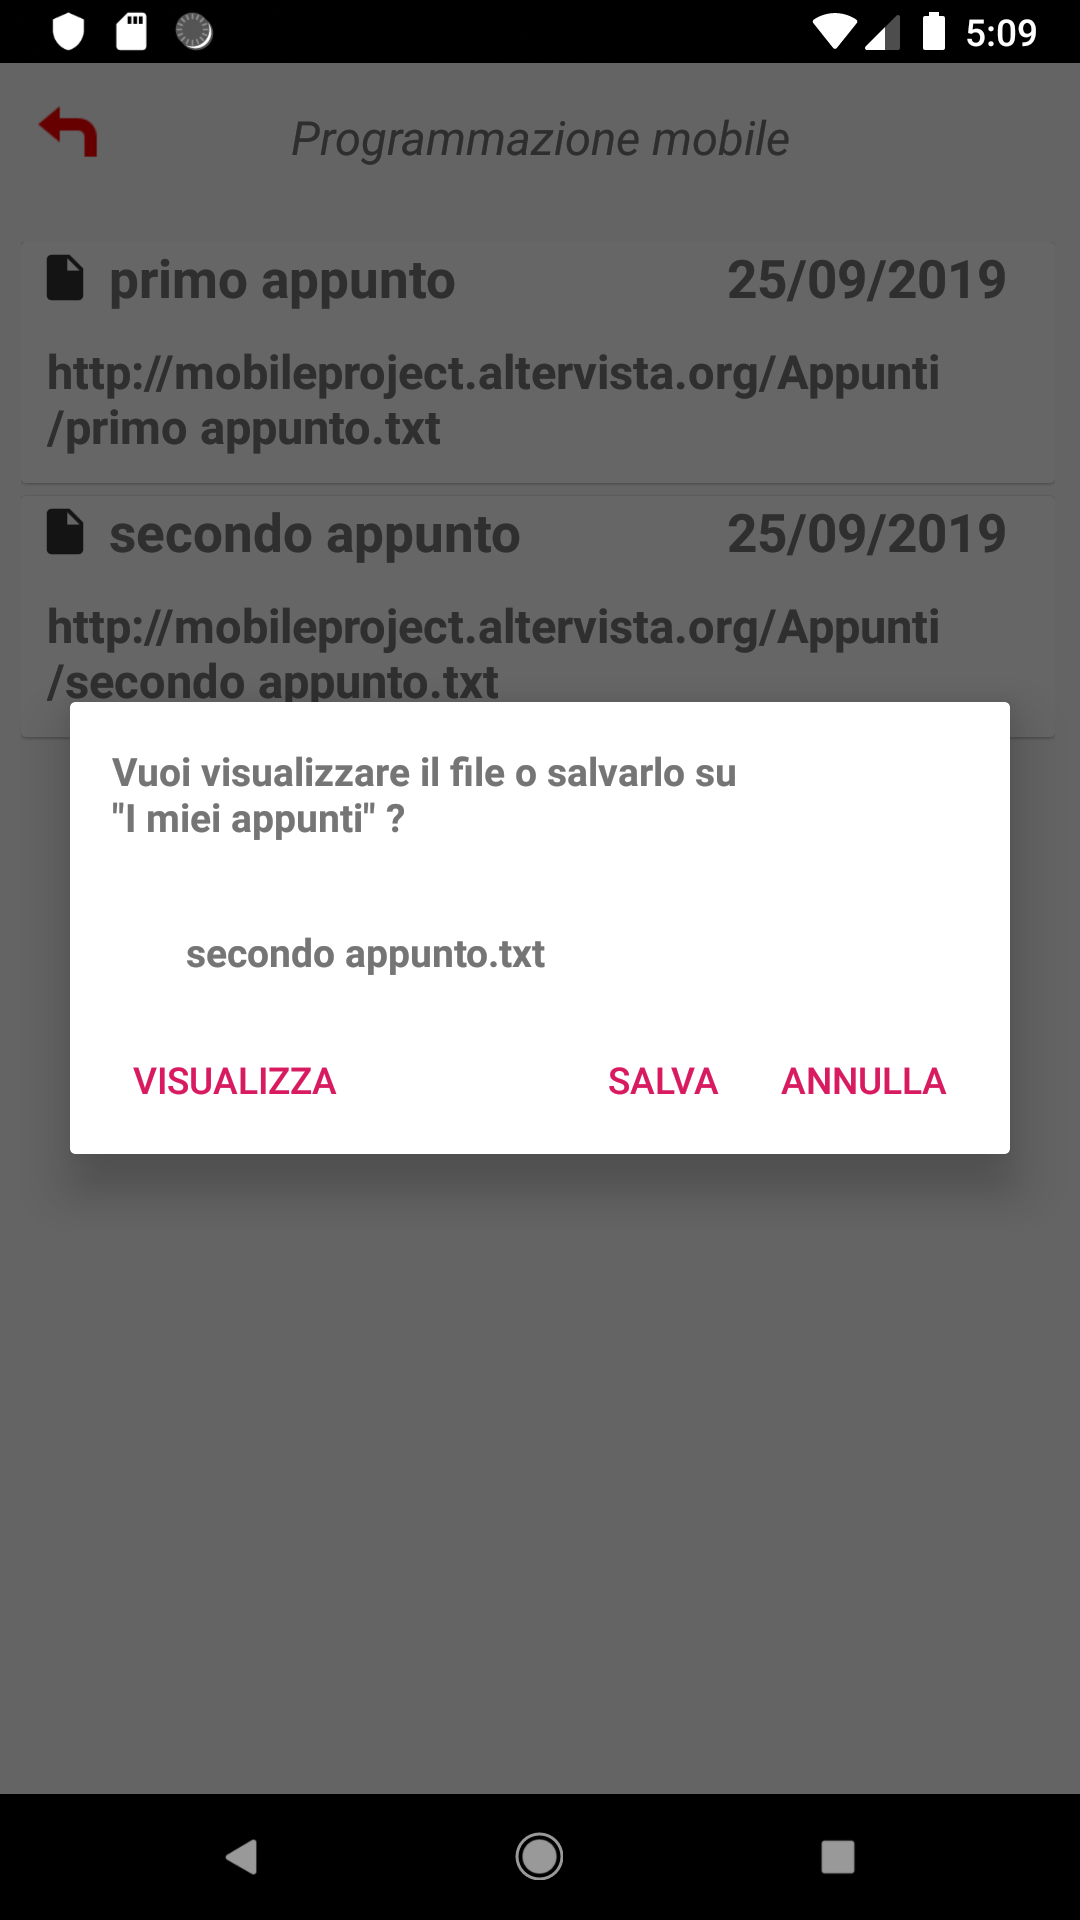
\includegraphics[width=.30\textwidth]{appunti_condivisi_scegli_azione}}
	\caption{\small Appunti condivisi, scegli la materia, scegli l'appunto, visualizza o scarica.}
\end{figure}

\subsection{Impostazioni}
Dalle impostazioni possiamo banalmente modificare \textbf{username}, \textbf{password} e leggere informazioni \textbf{about us}.

\begin{figure}[!h]
	\centering
	{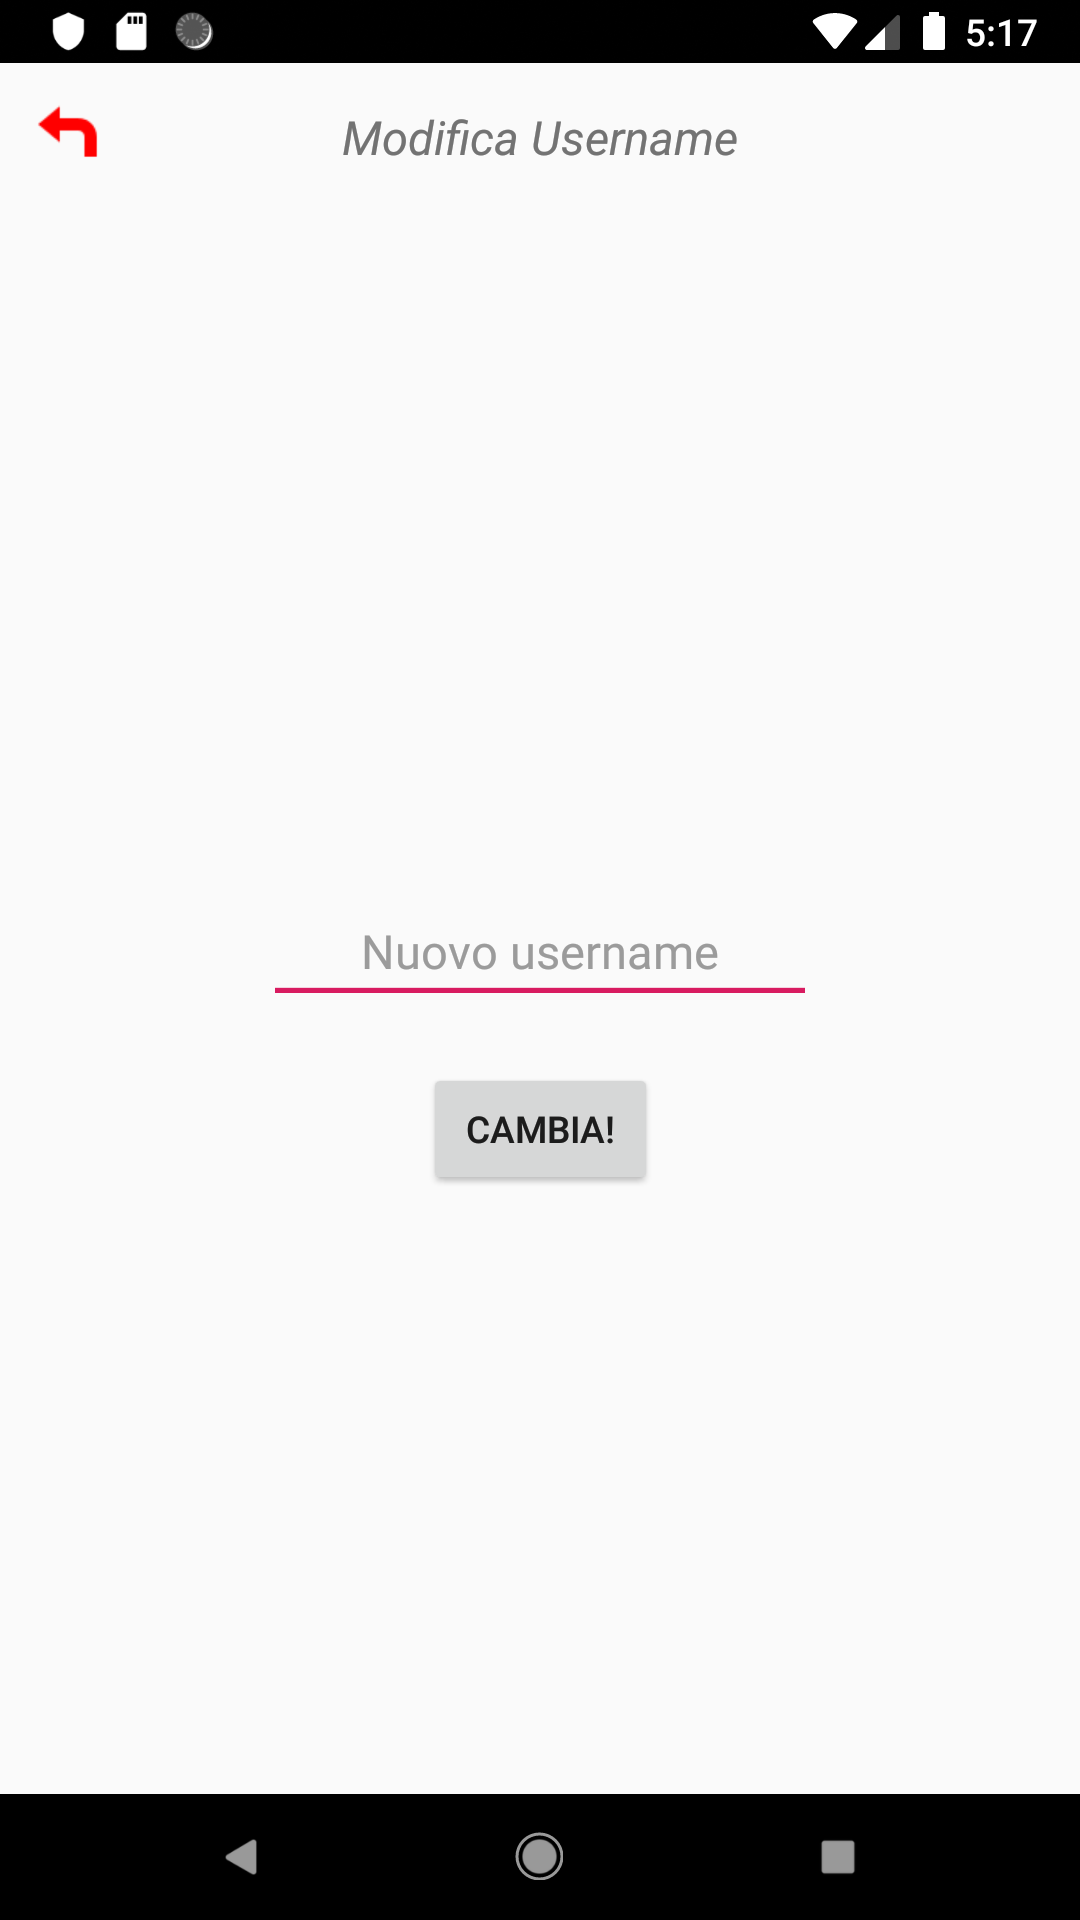
\includegraphics[width=.30\textwidth]{impostazioni_username}} \quad
	{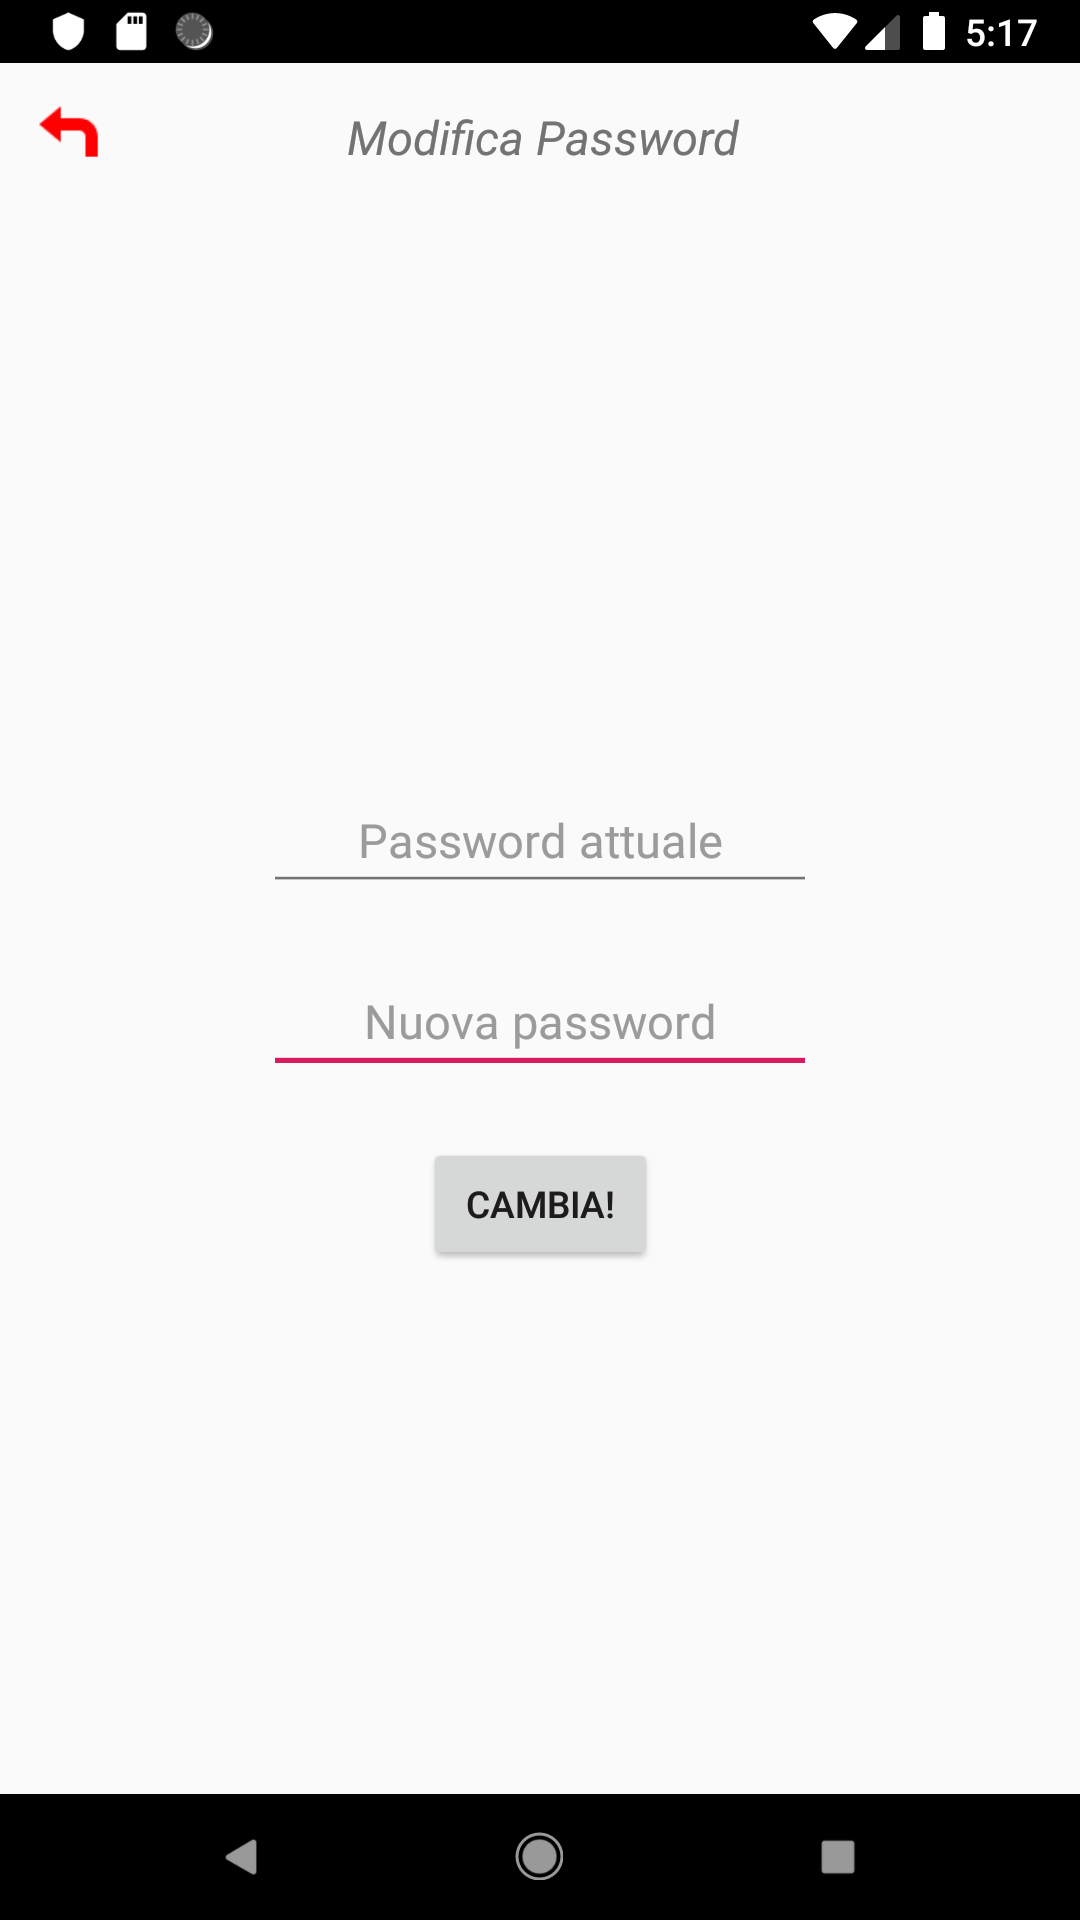
\includegraphics[width=.30\textwidth]{impostazioni_password}} \quad
	{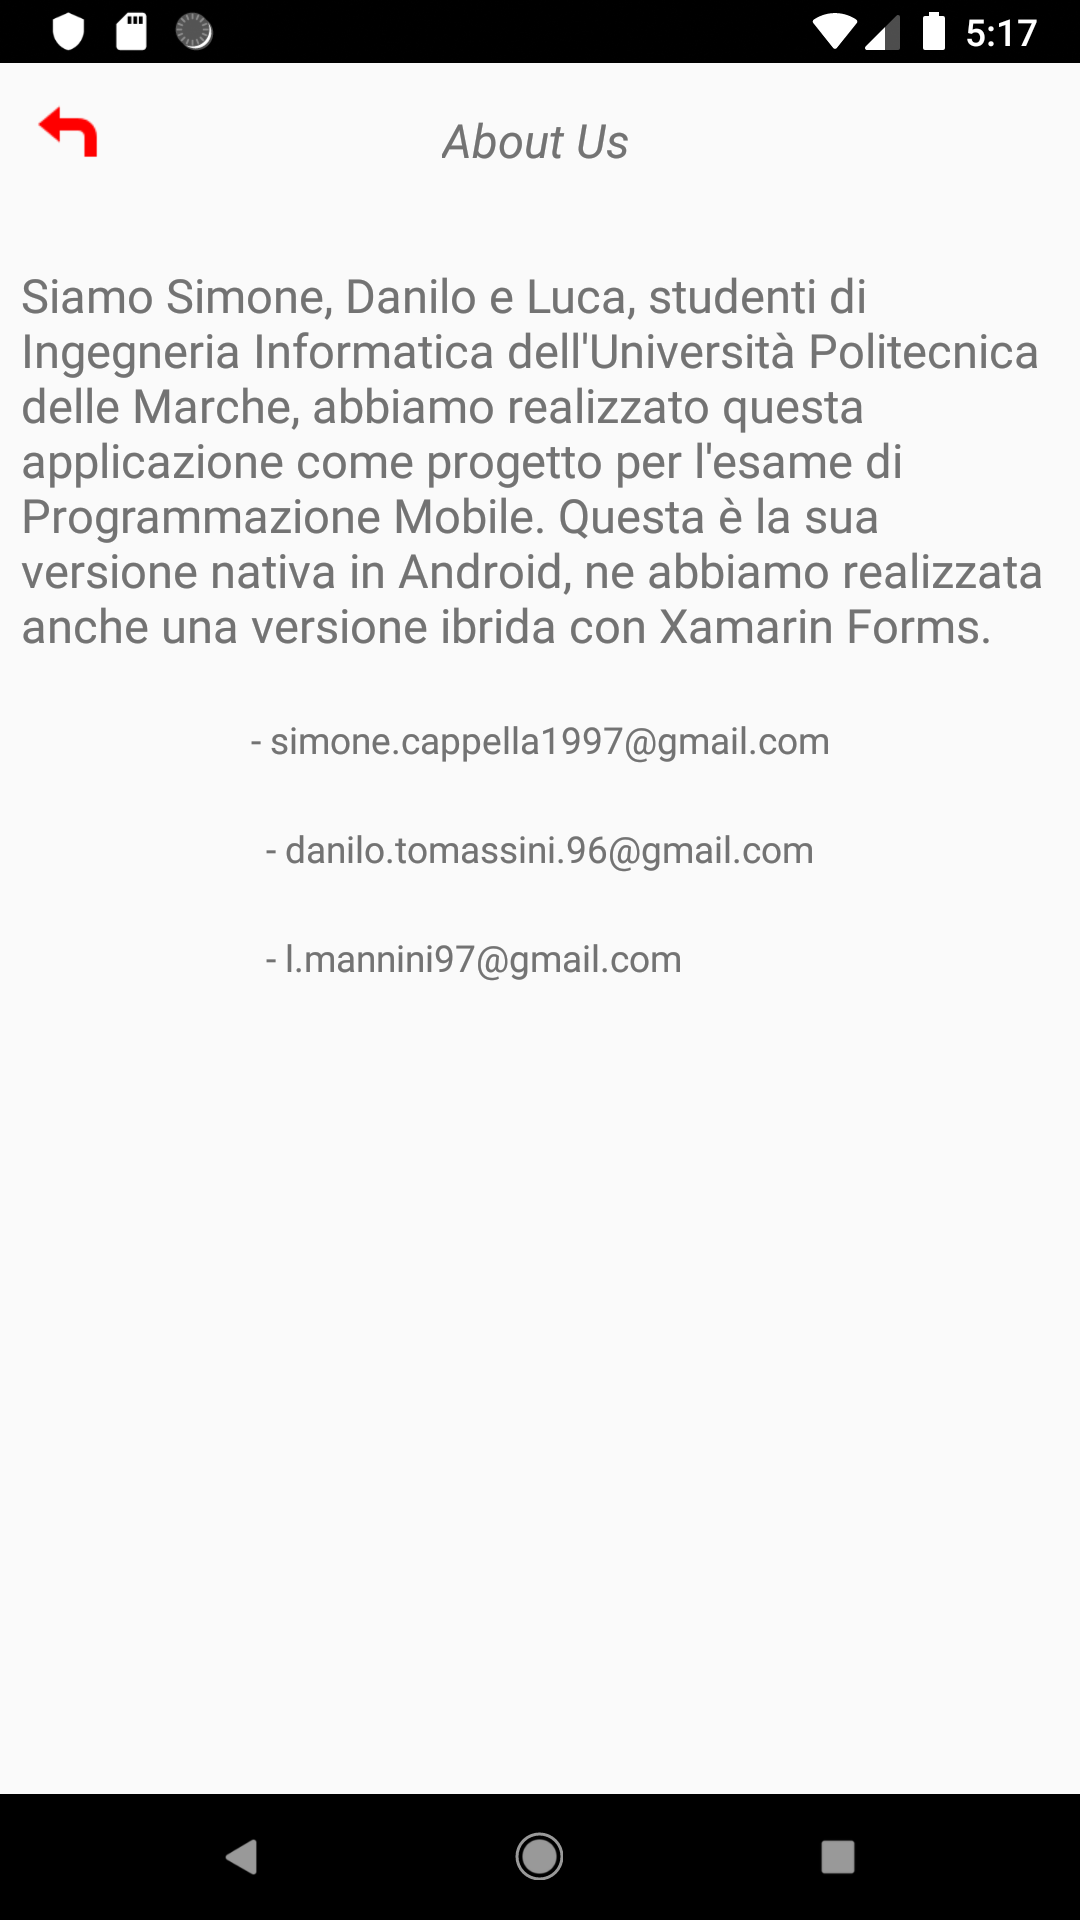
\includegraphics[width=.30\textwidth]{impostazioni_about_us}}
	\caption{\small Azioni eseguibili nelle impostazioni.}
\end{figure}
\newpage 
\section{Implementazioni Android studio}
\subsection{Classe SupportTask}
Riteniamo opportuno introdurre questa classe e le sue funzionalità ad inizio capitolo poichè essa verrà utilizzata da tutte le funzionalità che richiedono un accesso al database degli utenti. 

Notiamo subito che la nostra classe estende la classe astratta \textbf{AsyncTask}. Innanzitutto definiamo il significato di task asincrona: una task asincrona è un metodo che non va a lavorare sul thread principale del programma, per cui quest'ultimo può proseguire senza attendere che il metodo chiamato terminati. Nel costruttore inizializziamo il contesto relativo alla classe chiamante. Dal momento che estendiamo una classe astratta dobbiamo sovrascrivere i metodi che ci interessano. Il metodo che andiamo a sovrascrivere noi è $doInBackground$ che rappresenta la vera e propria logica del metodo. Non passiamo un numero definito di variabili a tale metodo poichè essi dipenderanno da quale classe del nostro programma effettuerà la chiamata. Vengono utilizzati i tre puntini per indicare che ciò che esso riceverà come parametro sarà un array di stringhe, di nome $params$, di grandezza appunto indefinita. I valori in tale array verrano memorizzati secondo l'ordine in cui vengono inseriti nei parametri al momento della chiamata del metodo. Verrano quindi recuperati accedendo all'indice corrispondente alla posizione del valore nei parametri di chiamata. Il primo parametro che passiamo a questo metodo è sempre $method$, ovvero una stringa sulla quale andremo ad effettuare vari controlli per capire cosa l'utente ha richeisto. 
\begin{lstlisting}
\\SupportTask\\
public class SupportTask extends AsyncTask <String, Void, String> {
    Context ctx;

    SupportTask(Context ctx) {
        this.ctx = ctx;
    }

    protected void show(String message) {
        Toast.makeText(ctx, message, Toast.LENGTH_LONG).show();
    }

    @Override
    //Ricevo i parametri in un array di dimensione variabile
    protected String doInBackground(String... params) {
        String line;
        String method = params[0];
[...]
\end{lstlisting}
Prenderemo in esame soltanto il caso in cui l'utente chieda di registrarsi, gli altri casi sono gestiti in maniera praticamente analoga se non per il numero di parametri che riceviamo e che inviamo al server. 

Andiamo ad impostare la connessione, tramite l'oggetto \textbf{HttpURLConnection}, e il metodo con il quale invieremo i dati della form. Produciamo poi la stringa che comporrà il body del messaggio al server secondo le regole del metodo post, ovvero "nome\_variabile1"=valore1 \&  "nome\_variabile2"=valore2. Vengono inviati i dati e viene chiuso lo stream. Per leggere la risposta del server utilizziamo l'oggetto \textbf{InputStream} e il \textbf{BufferedReader}, salviamo tutto nella stringa $state$ e la ritorniamo alla classe chiamante andando ad invocare il metodo \textbf{trim()} che elimina eventuali spazi bianchi all'inizio della stringa.
\begin{lstlisting}
\\SupportTask\\
if (method.equals("register")) {
            String state = "";
            String user_name = params[1];
            String user_pass = params[2];
            String reg_url = params[3];
            try {
                URL url = new URL(reg_url);
                //mi connetto all'URL al quale effettuare la richiesta, 
impostando anche il tipo di richiesta
                HttpURLConnection httpURLConnection = (HttpURLConnection) 
url.openConnection();
                httpURLConnection.setRequestMethod("POST");
                httpURLConnection.setDoOutput(true);
                httpURLConnection.setDoInput(true);
                OutputStream OS = httpURLConnection.getOutputStream();
                BufferedWriter bufferedWriter = new 
BufferedWriter(new OutputStreamWriter(OS, "UTF-8"));
                //Creo la stringa che compone la richiesta
                String data = URLEncoder.encode("user_name", "UTF-8") + "=" 
+ URLEncoder.encode(user_name, "UTF-8") + "&" +
                        URLEncoder.encode("user_pass", "UTF-8") + "=" 
+ URLEncoder.encode(user_pass, "UTF-8");
                bufferedWriter.write(data);
                bufferedWriter.flush();
                bufferedWriter.close();
                OS.close();
                InputStream IS = httpURLConnection.getInputStream();
                BufferedReader bufferedReader = new 
BufferedReader(new InputStreamReader(IS, "iso-8859-1"));
                while((line = bufferedReader.readLine()) != null)
                {
                    state += line;
                }
                bufferedReader.close();
                IS.close();
                httpURLConnection.disconnect();
            } catch (MalformedURLException e) {
                e.printStackTrace();
            } catch (IOException e) {
                e.printStackTrace();
            } return state.trim();
[...]
\end{lstlisting}
\subsection{Login e Registrazione}
Per avviare il login, ovviamente, è necessario riempire le \textbf{EditText} relative a username e password; i relativi valori verranno assegnati alle variabili \textbf{login\_name} e \textbf{login\_pass}.

La connessione al database viene instaurata indicando \textbf{method}, stringa inizializzata in precedenza a \textbf{"login"}, dati relativi ad username e password e l'url contenente il percorso fino alla funzione di login contenuta nel server.

Se la funzione del server da esito negativo non verrà effettuato il login e verrà stampato un \textbf{Toast}, per mezzo della funzione \textbf{show}. Altrimenti verrà stampato un messaggio di benvenuto e verrà lanciata la \textbf{MainActivity}.
\begin{lstlisting}
\\FirstActivity\\
[...]
public void userLogin(View view) {
[...]
try {
	Sring url = "http://mobileproject.altervista.org/login.php";
	auth = supportTask.execute(method, login_name, login_pass, url).get();
	} catch (ExecutionException e)
	{
		e.printStackTrace();
	}catch (InterruptedException a)
	{
		a.printStackTrace();
	}
	if(auth.equals("Login Success"))
	{
		launchMainActivity(view);
		show("Benvenuto "+ login_name + "!");
		finish();
	}else
	{
		show("Dati errati. Riprova.");
	}
}
[...]
\end{lstlisting}
Il codice PHP relativo alla funzione di login è mostrato di seguito.
\begin{lstlisting}
<?php
 require 'init.php';
 $user_name = $_POST["login_name"];  
 $user_pass = $_POST["login_pass"];  
 $sql_query = "SELECT * FROM Utenti WHERE username = '$user_name' AND 
password = '$user_pass'";  
 $result = mysqli_query($con,$sql_query);  
 if(mysqli_num_rows($result)> 0)  
 {    
 echo "Login Success";  
 }  
 else  
 {
 echo "Login Failed";  
 }  
 ?>
\end{lstlisting}
La registrazione viene gestita in modo simile.

In un \textbf{if} viene verificato in modo veloce se le condizioni su username e password sono verificate, in caso contrario viene lanciato un avviso.
Il metodo con cui si instaura la connessione al server è lo stesso, cambiano solo gli argomenti, \textbf{url} e \textbf{method}.Una volta che la registrazione è andata a buon fine l'attività viene interrotta e si torna alla schermata di login.
\begin{lstlisting}
\\Register\\
[...]
public void userRegister() {
[...]
if (register_name.length() >= 3 && register_pass.length() >= 3)
{
	try {
		String url = "http://mobileproject.altervista.org/register.php";
		auth= supportTask.execute(method, register_name, register_pass, url).get();
	} catch (ExecutionException e) {
		e.printStackTrace();
	} catch (InterruptedException e) {
		e.printStackTrace();
	}
	if (auth.equals("Registrazione avvenuta con successo!")) {
		show("Registrazione effettuata con successo, accedi!");
		finish();
	} else if (auth.equals("Username in uso")) {
		show("Username gia' in uso, prova con uno diverso!");
	}
}
else
{
show(I campi devono contenere almeno 3 caratteri.);
}
[...]
\end{lstlisting}
Di seguito abbiamo inserito il codice PHP relativo alla funzione di registrazione.
\begin{lstlisting}
<?php
 require "init.php";
 
 $user_name = $_POST["user_name"];  
 $user_pass = $_POST["user_pass"];
 $ver = "SELECT * FROM Utenti WHERE username = '$user_name' ";
 $result = mysqli_query($con,$ver);
 $row = mysqli_fetch_array($result,MYSQLI_NUM);
 if ($row[0] > 0)
 	{
    echo "Username in uso";
    }
    else{
 			$sql_query = "INSERT INTO Utenti (username,password) 
values('$user_name','$user_pass')";
 			if(mysqli_query($con,$sql_query))
 				{
    				echo"Registrazione avvenuta con successo!";
				}else
    				echo"Errore";
          }
 ?>
\end{lstlisting}
\subsection{Orario}
Avviata l'activity \textbf{orario} vengono catturate le dimensioni del display, calcolata la dimensione del \textbf{fragment} contenente la tabella dell'orario e fatto partire uno switch sul giorno corrente.

\begin{lstlisting}
\\Clock\\
[...]
protected void onCreate(Bundle savedInstanceState) {
[...]
Calendar calendar = Calendar.getInstance();
int day = calendar.get(Calendar.DAY_OF_WEEK);
Fragment fragment = null;
switch (day){
	case Calendar.MONDAY:
		fragment = new lun_fragment();
		nav.setSelectedItemId(R.id.lun);
		break;
	case Calendar.TUESDAY:
		fragment = new mar_fragment();
		nav.setSelectedItemId(R.id.mar);
		break;
	case Calendar.WEDNESDAY:
[...]
}
loadFragment(fragment);
[...]
\end{lstlisting}

Questo switch permette di caricare il fragment relativo al giorno corrente (es. se oggi è lunedì viene caricato il fragment relativo a lunedì); viene, infatti, inizializzato l'oggetto fragment e viene selezionato l'elemento sulla navbar.

\begin{lstlisting}
\\Clock\\
[...]
public boolean onNavigationItemSelected(@NonNull MenuItem item) {
Fragment fragment = null;
switch(item.getItemId())
{
	case R.id.lun:
		next = 0;
		fragment = new lun_fragment();
		break;
	case R.id.mar:
		next = 1;
		fragment = new mar_fragment();
		break;
	case R.id.mer:
		next = 2;
		fragment = new mer_fragment();
		break;
[...]
}
return loadFragment(fragment);
[...]
\end{lstlisting}

Allo stesso modo la funzione \textbf{onNavigationItemSelected}, associa in base allitem della navbar cliccato un'istanza del fragment all'oggetto fragment e nuovamente viene lanciata la funzione \textbf{loadFragment}.

La funzione \textbf{loadFragment} carica il fragment richiesto e gestisce lo scorrimento a destra o sinistra dipendentemente dalla posizione del fragment corrente rispetto a quello scelto.
\begin{lstlisting}
private boolean loadFragment(android.support.v4.app.Fragment fragment)
    {
        if(fragment!= null)
            {
            FragmentTransaction ft = 
getSupportFragmentManager().beginTransaction();
            if(curr < next)
                {
                    ft.setCustomAnimations(R.anim.slide_in,R.anim.slide_out);
                }else
                    {
                        ft.setCustomAnimations(R.anim.slide_in_left,
R.anim.slide_out_right);
                    }
            curr = next;
            ft.replace(R.id.fragment_container, fragment);
            ft.commit();
            return true;
        }
        return false;
    }
\end{lstlisting}
\subsubsection{Gestione orario}
Prendiamo come riferimento il fragment relativo al \textbf{lunedì}, gli altri saranno implementati in modo analogo.

All'interno del fragment vengono nuovamente catturate le dimensioni del display e impostate le dimensioni delle varie caselle della tabella, rispettivamente:
\begin{itemize}
\item \textbf{Ora:} l'ora di inizio della lezione.
\item \textbf{Materia:} la materia inserita.
\item \textbf{Aula:} l'aula nel quale si terrà la lezione.
\item \textbf{X:} edit per cancellare la riga.
\end{itemize}

La tabella viene inizializzata nella funzione \textbf{onCreate}, qui, ogni elemento della tabella viene assegnato ad una variabile e successivamente "riempito" con il testo salvato, andadolo a recuperare con l'oggetto \textbf{sa}, della classe \textbf{SalvaOrario}, passando la chiave $\{lun\_1, lun\_2,..., lun\_11\}$ per quanto riguarda la tabella di lunedì, per la tabella di martedì le chiavi saranno costruite come $\{mar\_1,...,mar\_11\}$; la stessa logica vale per gli altri giorni; in tal modo possiamo recuperare in modo distinto le 11 materie salvate con la relativa aula per i diversi giorni.

\begin{lstlisting}
\\lun_fragment\\
[...]
public View onCreateView(LayoutInflater inflater, 
@Nullable ViewGroup container, @Nullable Bundle savedInstanceState) {
[...]
SalvaOrario sa = new SalvaOrario();
[...]
txtMat1 = v.findViewById(R.id.materia1);
txtMat1.setText(sa.getMateria("lun_1", getActivity()));
txtMat1.setOnClickListener(this);
txtAula1 = v.findViewById(R.id.aula1);
txtAula1.setText(sa.getAula("lun_1", getActivity()));
txtOra1 = v.findViewById(R.id.ora1);

txtMat2 = v.findViewById(R.id.materia2);
txtMat2.setText(sa.getMateria("lun_2", getActivity()));
txtMat2.setOnClickListener(this);
txtAula2 = v.findViewById(R.id.aula2);
txtAula2.setText(sa.getAula("lun_2", getActivity()));
txtOra2 = v.findViewById(R.id.ora2);
[...]
\end{lstlisting}

Nella funzione \textbf{onClick} viene gestita la scelta di inserire una materia nell'orario o eliminarne una dallo stesso. C'è, infatti, uno switch che gestisce il "click" nelle diverse sezioni della tabella. Abbiamo due diversi tipi di azione:
\begin{itemize}
\item \textbf{Aggiungere una materia:} per aggiungere una materia si seleziona un campo materia relativo all'ora in cui vogliamo inserirlo, questo attiverà l'elemento corrispondente nello switch che imposterà la variabile $n$, utilizzata successivamente per costruire la chiave e salvare nella classe SalvaOrario, la variabile $ora$, presa direttamente dalla view e chiama la funzione \textbf{launchList()}.
\item \textbf{Elimina una materia:} se viene selezionata la "X" sulla destra della tabella viene semplicemente "pulita" la riga corrispondente, infatti, nello switch, captato l'$edit$ corrispondente, viene impostata di nuovo la variabile $n$ per essere usata come chiave e le voci $materia$ e $aula$ vengono messe a $null$, viene lanciata, poi, la funzione \textbf{inserisciSalva()}; (la variabile $inc$ serve successivamente per inserire in un colpo solo più ore della stessa materia).
\end{itemize}
\newpage
\begin{lstlisting}
\\lun_fragment\\
[...]
public void onClick (View v) {
switch (v.getId())
{
	case R.id.materia1:
		n = 1;
		ora = txtOra1.getText().toString();
		v.startAnimation(buttonClick);
		launchList();
		break;
	case R.id.materia2:
		n = 2;
		ora = txtOra2.getText().toString();
		v.startAnimation(buttonClick);
		launchList();
		break;
[...]
	case R.id.edit1:
		n = 1;
		v.startAnimation(buttonClick);
		materia = null;
		aula = null;
		inc = 1;
		inserisciSalva();
		break;
	case R.id.edit2:
		n = 2;
		v.startAnimation(buttonClick);
		materia = null;
		aula = null;
		inc = 1;
		inserisciSalva();
		break;
[...]
\end{lstlisting}

La finzione \textbf{launchList}, chiamata nel momento in cui si vuole aggiungere una materia all'orario non fa altro che lanciare un \textbf{intent esplicito}, questo ci permette di scambiare dati tra l'activity chiamante e la chiamata, infatti tra i parametri della funzione \textbf{putExtra} abbiamo una chiave, $giorno\_ora$ e un valore, $"lunedi'" + ora$ ($ora$ è stata assegnata in precedenza nello switch). Inoltre c'è bisogno di un $REQUEST\_CODE$ utilizzato come chiave di riconoscimento tra le activity.

\begin{lstlisting}
\\lun_fragment\\
[...]
public static final int REQUEST_CODE = 0000;
[...]
public void launchList() {
	Intent intent = new Intent (getActivity(), List.class);
	intent.putExtra("giorno_ora", "lunedi'  " + ora);
	startActivityForResult(intent, REQUEST_CODE);
}
\end{lstlisting}

L'activity \textbf{List} genera la lsita predefinita delle materie da cui si può scegliere quella da inserire nella casella dell'orario scelta.

Qui i dati vengono recuperati proprio grazie alla chiave $giorno\_ora$, successivamente vengono istaziati $myDialog$ e $adapter$.

La funzione \textbf{setOnItemClickListener} chiamata per mezzo dell'oggetto $listMaterie$ e la successiva \textbf{OnItemClick} permettono di captare quale materia della lista viene scelta grazie alla sua posizione nella lista stessa.

Scelta la materia viene aperta la finestra di dialogo, all'interno di questa vengono definiti diversi elementi come una editText per l'aula e due bottoni, $- +$, questi permettono di incrementare e decrementare le ore di lezione relative alla materia.

Una volta inserita l'aula e il numero di ore si provede al salvataggio. Un listener sul bottone $btnSalva$ fa si che quando venga restituito il risultato all'activity chiamante con la variabile $intent$, questa contiene la materia scelta, l'aula e la conta delle ore, l'attivity termina con finish().
Una cosa analoga avviene nel momento in cui si decide tramite l'apposito bottone di inserire una nuova materia non contenuta nella lista predefinita.

\begin{lstlisting}
\\List\\
[...]
Intent intent = getIntent();
String giorno_ora = intent.getStringExtra("giorno_ora");
[...]
myDialog = new Dialog(this);
final ArrayAdapter<String>  adapter = new ArrayAdapter<>(this,
android.R.layout.simple_list_item_1, android.R.id.text1, listItem);
listMaterie.setAdapter(adapter);
[...]
listMaterie.setOnItemClickListener(new AdapterView.OnItemClickListener() {
	@Override
	public void onItemClick(AdapterView<?> parent, View view, int position,
	long id) {
		value = adapter.getItem(position);
[...]
myDialog.show();
[...]
btnMeno.setOnClickListener(new View.OnClickListener() {
	@Override
	public void onClick(View v) {
		i--;
		textContatore.setText(Integer.toString(i));
	}
}
[...]
btnPiu.setOnClickListener(new View.OnClickListener() {
	@Override
	public void onClick(View v) {
	i++;
	textContatore.setText(Integer.toString(i));
	}
}
[...]
btnSalva.setOnClickListener(new View.OnClickListener() {
	@Override
	public void onClick(View v) {
[...]
		Intent intent = new Intent();
		intent = intent.putExtra("mat", valore);
		setResult(Activity.RESULT_OK, intent);
		finish();
		myDialog.dismiss();
	}
[...]
\end{lstlisting}

La funzione \textbf{onActivityResult} si occupa di reperire dall'activity Lsit i risultati ottenuti dalla scelta. L'array di stringhe $res$ contiene ora nella posizione 0 la materia, nella posizione 1 l'aula e nella posizione 2 il numero di ore, che va "parsato" in un intero in quanto arrivava come una Stringa.

Viene considerato il caso in cui non si completa la scelta, in tal caso nell'activity Lista viene impostato il nome della materia a $back$ e non viene eseguita nessun'altra azione, la routine si interrompe. Nel caso in cui la scelta è stata completata i dati raccolti andranno salvati, sono passati, dunque, alla funzione \textbf{salvaOrario}.

\begin{lstlisting}
\\lun_fragment\\
[...]
public void onActivityResult(int requestCode, int resultCode, Intent data){
	super.onActivityResult(requestCode, resultCode, data);
	if ((requestCode == REQUEST_CODE) && (resultCode == Activity.RESULT_OK)) {
		String[] res = data.getStringArrayExtra("mat");
		materia = res[0];
		aula = res[1];
		inc = Integer.parseInt(res[2]);
	}
	if (materia.equals("back")){}
	else{
		salvaOrario(i, materia, aula);
	}
}
[...]
\end{lstlisting}

La funzione \textbf{salvaOrario} va a definire un cursore che sarà popolato con l'elemento del database trovato dal metodo \textbf{searchM} (questo trova nel database l'elemento il cui campo materia ha lo stesso nome della materia inserita).
Questo cursore permette di verificare, grazie all'$if$ se la materia inserita è gia presente nel database contenente le materie, in caso positivo il vecchio elemento viene eliminato; successivamente si inserisce nel database delle materie il nuovo elemento e viene chiamata la funzione \textbf{inserisciSalva()}.

Le materie vengono inserite nel database delle materie per permettere alla sezione $miei appunti$ di rendere disponibili le materie inserite nell'orario.

\begin{lstlisting}
\\lun_fragment\\
[...]
public void salvaOrario (String key, String materia, String aula) {
	Cursor c;
	c = dm.searchM(materia);
	if (c.getCount() > 0) {
		dm.delete(materia);
	}
	dm.insert(materia, ora, aula, key);
	inserisciSalva();
[...]
\end{lstlisting}

La funzione \textbf{inserisciSalva} permette di salvare, nuovamente tramite i metodi della classe \textbf{Salva Orario}, materia e aula scelti e nuovamente di aggiornare i valori delle $txtMat$ e $txtAula$.

Il \textbf{while} all'interno della funzione ripete il ciclo finchè la variabile $inc$ che conteneva la conta delle ore non arriva a 0; la Stringa $q$ viene costruita in modo da diventare una chiave per i metodi della classe SalvaOrario, infatti la variabile $i$ contiele la stringa "lun\_" e la variabile $n$ contiene il numero dipendentemente dalla riga scelta dalla tabella. Le variabili $n$ ed $inc$ alla fine del ciclo vengono rispettivamente incrementata e decrementata, questo permette di salvare in un solo colpo stessa materia e stessa aula all'interno della tabella, infatti il numero dell'elemento della tabella incrementa finche non si esaurisce il numero di ore deciso nella finestra di dialogo nell'activity List.

Lo \textbf{switch} su $n$ ha il compito di aggiornare immediatamente il valore della tabella nella posizione $n$.
\begin{lstlisting}
\\lun_fragment\\
[...]
public void inserisciSalva(){
	while (inc > 0){
		String q = i + n;
		sa.setMateria(q, materia, getActivity());
		sa.setAula(q, aula, getActivity());
		switch (n){
			case 1:
				txtMat1.setText(sa.getMateria(q, getActivity()));
				txtAula1.setText(sa.getAula(q, getActivity()));
				break;
			case 2:
				txtMat2.setText(sa.getMateria(q, getActivity()));
				txtAula2.setText(sa.getAula(q, getActivity()));
				break;
[...]
	}
	n++;
	inc--;
}
[...]
\end{lstlisting}

La classe \textbf{SalvaOrario} gestisce salvataggio ed estrazione per mezzo delle \textbf{SharedPreferences} di materia e aula.

Al suo interno sono presenti, infatti, quattro metodi:
\begin{itemize}
\item \textbf{setMateria:} prende tra gli argomenti chiave e materia e va a salvare la materia con tale chiave.
\item \textbf{getMateria:} va ad estrarre dai salvataggi la materia corrispondente alla chiave di ricerca.
\item \textbf{setAula:} di nuovo prende tra gli argomenti chiave ed aula (in questo caso la chiave viene combinata con la stringa $"\_A"$ per caratterizzare le chiavi relative alle aule) salva, dunque, il nome dell'aula.
\item \textbf{getAula:} estrae l'aula dai salvataggi per mezzo della chiave combinata con la stringa di cui sopra.
\end{itemize}

\begin{lstlisting}
\\SalvaOrario\\
[...]
public static void setMateria(String key, String value,  Context context) {
	SharedPreferences.Editor editor = preferences.edit();
	editor.putString(key, value);
	editor.commit();
}
public static String getMateria(String key, Context context)
{
	return preferences.getString(key, null);
}
public static void setAula(String key, String value,  Context context) {
	SharedPreferences.Editor editor = preferences.edit();
	editor.putString(key+"_A", value);
	editor.commit();
}
public static String getAula(String key, Context context) {
	return preferences.getString(key+ "_A", null);
}
\end{lstlisting}

\newpage
\subsection{I miei appunti}
Avviata l'activity \textbf{i miei appunti} viene mostrata la lista delle materie salvate nell'applicazione, queste sono il risultato delle materie aggiunte nell'orario o eventualmente aggiunte nella sezione in questione.

All'avvio si definisce e istanzia un cursore che va ad estrarre tutti gli elementi dal database e con un $CursorAdapter$ va a popolare la lsita. Nuovamente viene utilizzato un $onItemClickListener$ che permette di catturare l'elemento dalla lista, viene, dunque, chiamata l'activity \textbf{Notes\_Page} con un intent passando il parametro $a$, stringa che contiene il nome della materia scelta.

\begin{lstlisting}
\\MyNotes\\
[...]
protected void onCreate(Bundle savedInstanceState) {
[...]
cursor = dm.selectAll();
[...]
adapter = new SimpleCursorAdapter(this, R.layout.list_mat, cursor, 
	fromColumns, viewsList, 0);
listMat.setAdapter(adapter);
listMat.setOnItemClickListener(new AdapterView.OnItemClickListener() {
	@Override
	public void onItemClick(AdapterView<?> parent, View view, 
		int position, long id) {
		Cursor c = adapter.getCursor();
		String a = c.getString(2);
		Intent i = new Intent(getApplication(), Notes_Page.class);
		i.putExtra("mat", a);
		startActivity(i);
	}
}
[...]
\end{lstlisting}

\subsubsection{Aggiungi una materia}
Possiamo aggiungere manualmente una nuova materia o, eventualmente, eliminarne una contenuta nel database attivando il relativo bottone. Viene lanciata con un intent esplicito l'activity \textbf{AggMaterie}; si utilizza un intent esplicito per permettere l'aggiornamento della lista una volta aggiunta o eliminata una materia dalla stessa. Nella funzione \textbf{onActivityResult}, infatti, appurata la validità del ritorno dall'activity si estrae il dato, $res$ contiene il nome della materia aggiunta, e definito un nuovo cursore $nc$ si applicano metodi quali \textbf{changeCursor} sull'adapter in modo da indicargli il nuovo cursore da utilizzare e la \textbf{notifyDataSetChanged}; in tal modo la lista verrà aggiornata.

\begin{lstlisting}
\\MyNotes\\
[...]
public static final int REQUEST_CODE2 = 2222;
[...]
private void launchAggMat() {
	Intent intent = new Intent(this, AggMaterie.class);
	intent.putExtra("app", "agg materie");
	startActivityForResult(intent, REQUEST_CODE2);
}
@Override
public void onActivityResult(int requestCode, int resultCode, Intent data){
	super.onActivityResult(requestCode, resultCode, data);
	if ((requestCode == REQUEST_CODE2) && (resultCode == Activity.RESULT_OK)) {
		String res = data.getStringExtra("res");
		Toast.makeText(getApplicationContext(), res, Toast.LENGTH_SHORT).show();
	}
	Cursor nc;
	nc = dm.selectAll();
	adapter.changeCursor(nc);
	adapter.notifyDataSetChanged();
}
[...]
\end{lstlisting}

L'activity \textbf{AggMaterie} consiste di una $editText$ e due bottoni, uno per salvare la materia inserita nella edit e una per eliminarla.
Nella funzione \textbf{onCreate} dell'activity AggMaterie viene "raccolto" l'intent.

Le funzioni relative al salvataggio ed eliminazione sono implementate direttamente nella funzione \textbf{onClick}, con uno switch sull'elemento della vista cliccato.
\begin{itemize}
\item \textbf{Salva:} viene estratta la stringa e istanziato un cursore; tramite il cursore si va a cercare nel database un elemento il cui campo materia sia uguale alla materia inserita, nell'\textbf{if} viene dunque controllato tramite il metodo \textbf{getCount} sul cursore se tale elemento è stato trovato o meno, in caso positivo viene solo lanciato un avviso, altrimenti può essere salvata la nuova materia e terminata l'activity impostando il risultato dell'intent.
\item \textbf{Elimina:} si estrae nuovamente la stringa dalla edit, si istanzia il cursore e nuovamente si procede alla ricerca di un elemento il cui campo materia corrisponda alla materia scelta, stavolta nel caso in cui venga trovata viene eliminata e terminata l'activity.
\end{itemize}

\begin{lstlisting}
\\AggMaterie\\
[...]
protected void onCreate(Bundle savedInstanceState) {
[...]
	Intent intent = getIntent();
}
[...]
@Override
public void onClick(View v) {
	switch (v.getId()){
[...]
		case R.id.btnInsert:
			materia = editMateria.getText().toString();
			Cursor c = dm.searchM(materia);
			if(c.getCount() > 0){
				[...]
			}else{
				dm.insert(materia, "ora", "aula", "code");
				Intent res  = new Intent();
				res = res.putExtra("res", materia);
				setResult(Activity.RESULT_OK, res);	
				finish();
			}
			break;
		case R.id.btnDelete:
			String materia = editMateria.getText().toString();
			Cursor del = dm.searchM(materia);
			if (del.getCount() > 0){
				dm.delete(materia);
				finish();
			}
			[...]
			break;
	}
}
[...]
\end{lstlisting}

\subsubsection{Vedi appunti}
Scelta la materia dalla lista visualizzata all'avvio di \textbf{MyNotes} viene lanciata, come visto, l'activity \textbf{Notes\_Page}.

All'avvio viene subito estratto il dato passato dall'activity chiamante, si tratta del nome della materia scelta, successivamente vengono definiti un \textbf{cursore} che contiene gli elementi del database la cui materia coincide con quella ricevuta in $a$ e un \textbf{adapter} che permette di riempire la lista con gli elementi del cursore, in particolare vengono messi nella lista titolo e data dell'appunto.

\begin{lstlisting}
\\Notes_Page\\
[...]
protected void onCreate(Bundle savedInstanceState) {
	[...]
	Intent r = getIntent();
	a = r.getStringExtra("mat");
	[...]
	cursor = da.searchM(a);
	adapter = new SimpleCursorAdapter(this, R.layout.list_app_loc, cursor,
		fromColumns, viewsList, 0);
	listNote.setAdapter(adapter);
	[...]
\end{lstlisting}

In tal caso abbiamo due possibili eventi sulla lista, un click singolo o un click prolungato (longClick).
\begin{itemize}
\item \textbf{Click:} la funzione \textbf{onItemClick} gestisce il click singolo sull'elemento, grazie alla posizione viene istanziato un nuovo cursore all'elemento in questione e ne vengono estratti come stringhe $materia, titolo, data e l'appunto vero e proprio$, viene, dunque, stampato a schermo un \textbf{Toast} contenente il titolo dell'appunto scelto e viene lanciata la funzione \textbf{launchVedi}.
\item \textbf{LongClick:} il long click permette di eliminare l'appunto. Viene nuovamente istanziato un cursore attraverso il quale vado ad estrarre $code$ e $titolo$ dell'appunto selezionato.

Viene successivamente costruita una finestra di dialogo grazie alla classe AlertDialog. Nell'alert dialog devono essere settati i bottoni "positivo" e "negativo", rispettivamente grazie a \textbf{setPositiveButton} e \textbf{setNegativeButton}.

Settato il positive button al suo interno viene utilizzata una funzione \textbf{onClick} che al click fa partire il metodo \textbf{delete} della classe \textbf{DataAppLoc}, database per gli appunti, che va a cancellare l'appunto andandolo a cercare con la variabile $code$. Successivamente viene aggiornata la lista come nelle activity precedenti e costruita la stringa con il percorso del file questo viene cancellato.

Il set del negative button non implementa nessuna funzione, in tal caso la alert dialog viene chiusa.
\end{itemize}

\begin{lstlisting}
\\Notes_Page\\
[...]
da = new DataAppLoc(this);
[...]
listNote.setOnItemClickListener(new AdapterView.OnItemClickListener() {
	@Override
	public void onItemClick(AdapterView<?> parent, View view, int position,
		long id) {
		Cursor c = adapter.getCursor();
		code = c.getString(0);
		String materia = c.getString(1);
		String titolo = c.getString(3);
		String data = c.getString(2);
		String app = c.getString(4);
		Toast.makeText(getApplicationContext(), code, Toast.LENGTH_SHORT).show();
		launchVedi(materia, titolo, data, app);
	}
	@Override
	public boolean onItemLongClick(AdapterView<?> parent, final View view,
		final int position, long id) {
		Cursor c = adapter.getCursor();
		code = c.getString(0);
		final String titolo = c.getString(3);
		[...]
		LayoutInflater inflater = LayoutInflater.from(context);
		View mess = inflater.inflate(R.layout.messaggio_elimina,null);
		AlertDialog.Builder alertDialogBuilder = new AlertDialog.Builder(context);
		alertDialogBuilder.setView(mess);
		alertDialogBuilder.setPositiveButton("ELIMINA",
			new DialogInterface.OnClickListener() {
			@Override
			public void onClick(DialogInterface dialog, int which) {
				da.delete (code);
				Cursor nc;
				nc = da.searchM(a);
				adapter.changeCursor(nc);
				adapter.notifyDataSetChanged();
				Context context = getApplicationContext();
				String folder = context.getFilesDir().getAbsolutePath()
					+ File.separator + "Appunti/";
				File file = new File(folder + titolo + ".txt");
				boolean deleted = file.delete();
			}
		}
		alertDialogBuilder.setNegativeButton("ANNULLA",
			new DialogInterface.OnClickListener() {
			@Override
			public void onClick(DialogInterface dialog, int which) {}
		}
		[...]
\end{lstlisting}

Come già detto nel caso di un singolo click su un elemento della lista viene chiamata la funzione \textbf{launchVedi}, questa crea un intent e un bundle contenente nome della materia cui si riferisce, titolo dell'appunto, data e annotazioni, questo bundle viene inserito nell'intent con il quale sarà chiamata l'activity \textbf{VediAppunti}.

\begin{lstlisting}
\\Notes_Page\\
[...]
public void launchVedi(String materia, String titolo, String data, String app){
	Intent i = new Intent(getApplication(), VediAppunti.class);
	Bundle bundle = new Bundle();
	bundle.putString("materia", materia);
	bundle.putString("titolo", titolo);
	bundle.putString("data", data);
	bundle.putString("app", app);
	i.putExtra("data", bundle);
	startActivity(i);
}
\end{lstlisting}

Nel caso in cui si voglia aggiungere un appunto va attivato il bottone \textbf{Aggiungi}, il cui evento è catturato nella funzione \textbf{onClick} della classe; questa banalmente chiama la funzione \textbf{launchAggiungi}.

La funzione in questione si occupa semplicemente di utilizzare un intent esplicito che va a lanciare l'activity \textbf{AggiungiAppuntiLoc}

\begin{lstlisting}
\\Notes_Page\\
[...]
public void launchAggiungi(){
	Intent intent = new Intent(this, AggiungiAppuntiLoc.class);
	intent.putExtra("app", a);
	startActivityForResult(intent, REQUEST_CODE1);
}
[...]
\end{lstlisting}

L'activity \textbf{AggiungiAppuntiLoc} si occupa di salvare gli appunti in locale ed eventualmente nella sezione per gli appunti condivisi.

Per quanto riguarda il salvataggio in locale, nella funzione \textbf{onClick} della classe nel caso in cui venga attivato il bottone $salva$ vengono salvati i testi inseriti delle edit e i dati vengono salvati nel database relativo agli appunti, viene, quindi, restituito l'intent con la variabile $res$ con una semplice stringa $"Appunti salvati"$.

\begin{lstlisting}
\\AggiungiAppuntiLoc\\
[...]
public void onClick(View v) {
[...]
	case R.id.btnSalvaApp:
		final String titolo = editTitolo.getText().toString();
		String data = editData.getText().toString();
		String appunti = editApp.getText().toString();
		da.insert(a, data, titolo, appunti);
		String res = "Appunti salvati";
		Intent intent = new Intent();
		intent = intent.putExtra("res", res);
		setResult(Activity.RESULT_OK, intent);
[...]
\end{lstlisting}

Terminata l'activity per salvare nuovi appunti si torna alla Notes\_Page, qui la funzione \textbf{onActivityResult} come al solito controlla il risultato dell'activity chiamata con il $REQUEST\_CODE$ e il $RESULT\_OK$, verificata la validità viene stampato il messaggio per la conferma del salvataggio e successivamente aggiornata la view della lista.

\begin{lstlisting}
public void onActivityResult(int requestCode, int resultCode, Intent data){
	[...]
	if ((requestCode == REQUEST_CODE1) && (resultCode == Activity.RESULT_OK)) {
		String res = data.getStringExtra("res");
		Toast.makeText(getApplicationContext(), res, Toast.LENGTH_SHORT).show();
	}
	Cursor nc;
	nc = da.searchM(a);
	adapter.changeCursor(nc);
	adapter.notifyDataSetChanged();
}
[...]
\end{lstlisting}
\newpage
\subsection{Appunti condivisi}
\subsection{Impostazioni}
La sezione per le impostazioni è molto basilare. Le voci che vanno a comporre il suo menù sono tre: Modifica Username, Modifica Password e About Us. Il tutto viene gestito con una ListView. Quando viene effettuato un click su una delle tre voci viene lanciata l’activity corrispondente tramite la funzione \textbf{setOnItemClickListener} che associa all'oggetto $lv$, che è una \textbf{ListView}, un listener. Un listner è un gestore degli eventi, che cattura, in questo caso, il click su un item della nostra ListView. Come parametro è necessario passargli un oggetto \textbf{Listner} che andiamo a istanziare direttamente inline. Successivamente è necessario sovrascrivere il metodo \textbf{OnItemClick} fornitoci dall'interfaccia \textbf{AdapterView.OnItemClickListener} inserendo al suo interno la logica del nostro gestore eventi.

Il metodo \textbf{OnItemClick} ci viene in aiuto estrapolando dal click dell'utente il numero sequenziale dell'elemento della ListView cliccato ed inserendolo nella variabile intera $position$, ad esempio: se l'utente cliccherà sulla voce \textbf{Modifica Username}, che è la prima dall'alto, il valore di $position$ sarà pari a $0$. Lo \textbf{switch} gestisce i diversi casi chiamando la funzione apposita per l'apertura dell'activity desiderata.
\begin{lstlisting}
\\Settings\\
lv.setOnItemClickListener(new AdapterView.OnItemClickListener() {
	@Override
  public void onItemClick(AdapterView<?> parent, View view, int position,
  long id)
	{
        	switch(position)
                {
                	case 0:
                        	launchEditUser(view);
                       		break;
                	case 1:
                        	launchEditPass(view);
                        	break;
                        case 2:
                        	launchAboutUs(view);
                        	break;
                }
  }
\end{lstlisting}
\subsubsection{Modifica Username}
Activity minimal per quando riguarda la modifica dello username. Essa presenta una \textbf{EditText} nel quale inserire il nuovo username desiderato e un \textbf{Button} per eseguire l’operazione di modifica. Al click sul bottone parte una procedura che innanzitutto verifica se lo username inserito rispetta le condizioni sulla lunghezza del campo e che fa poi partire il metodo \textbf{execute} della classe \textbf{SupportTask} per effettuare la modifica vera e propria sui nostri database. Il codice php è strutturato in modo che ci ritorni delle stringhe che andremo a prendere e inserire nella variabile $auth$. Sulla base del valore di $auth$ verrano mostrati avvisi all’utente che andranno ad indicare se l’operazione è andata a buon fine o meno. Nel blocco \textbf{catch} vengono gestiti i casi in cui vengano lanciate delle eccezioni dal codice presente nel blocco \textbf{try}.
\begin{lstlisting}
\\EditUser\\
[...]
String method = "edit";
                String newusr = txtNewusr.getText().toString();
                String auth = "";
                SupportTask supportTask = new SupportTask(EditUser.this);
                if (newusr.length() >= 3)
                {
                    try
                    {
                        String url = "http://mobileproject.altervista.org/
editusername.php";
                        auth = supportTask.execute(method, FirstActivity.
login_name, newusr, url).get();
			FirstActivity.login_name = newusr;
                    }catch (ExecutionException e)
                    {
                        e.printStackTrace();
                    }catch (InterruptedException a)
                    {
                        a.printStackTrace();
                    }
                    switch(auth) {
                        case "modificato":
                            Toast.makeText(this, "Username cambiato con 
successo!", Toast.LENGTH_SHORT).show();
                            Toast.makeText(this, "Per cambiare nome nella home 
riavviare l'applicazione.", Toast.LENGTH_SHORT).show();
                            break;
                        case "in uso":
                            Toast.makeText(this, "Username in uso!", Toast.
LENGTH_SHORT).show();
                            break;
                        default:
                            Toast.makeText(this, "Errore, la preghiamo di 
riprovare in seguito.", Toast.LENGTH_SHORT).show();
                            break;
                    }
                }else
                {
                    Toast.makeText(this, "L'username deve essere minimo di 3 
caratteri.",Toast.LENGTH_SHORT).show();
                }
[...]
\end{lstlisting}
Il codice PHP è molto semplice, riceve tramite metodo POST due variabili, lo username attuale, e il nuovo username desiderato dall'utente. Effettua innanzitutto un controllo per verificare che le variabili ricevute non siano nulle, poi controlla che il nuovo username sia disponibile, in caso affermativo effettua la query di update al database stampando un risultato di modifica avvenuta.
\begin{lstlisting}
\\editusername.php\\
<?php 
require 'init.php';
$oldusername = $_POST['oldusername'];
$newusername = $_POST['newusername'];
$querycheck = "SELECT * FROM Utenti WHERE username = '$newusername'";
$querycheckold = "SELECT * FROM Utenti WHERE username = '$oldusername'";
$queryupdate = "UPDATE Utenti SET username = '$newusername' WHERE username = '$oldusername' ";
$result = mysqli_query($con, $querycheck);
$resultold = mysqli_query($con, $querycheckold);
$num = mysqli_num_rows($resultold);
//echo $num;
if($oldusername!= null && $newusername!= null)
{
	if(mysqli_num_rows($result) > 0)
    {
    	echo "in uso";
    }else if ($num == 1)
    	{	
        	mysqli_query($con, $queryupdate);
        	echo "modificato";
        } else
        	{
            	echo 'username attuale errato'; 
            }
}else
	{
    	echo "campi errati";
    }
?>
\end{lstlisting}
\subsubsection{Modifica Password}
Il funzionamento di tale sezione dell’applicazione è del tutto simile a quello per la modifica dello username. Anche qui, come in Modifica Username, è stato necessario recuperare l'username dell'utente attualmente loggato, per poter effettuare le query sul giusto record del database. Qui il nome utente viene recuperato direttamente dalla funzione \textbf{execute} accedendo alla variabile statica $login\_name$ che viene valorizzata non appena l'utente effettua il login. Una variabile statica è una variabile accessibile da ogni punto dell'applicazione per tanto potente quanto pericolosa. Riportiamo di seguito il codice PHP che si occupa della modifica della password.
\begin{lstlisting}
<?php
require 'init.php';
$username = $_POST['username'];
$oldpass = $_POST['oldpass'];
$newpass = $_POST['newpass'];
$querycheck = "SELECT * FROM Utenti WHERE username = '$username' AND 
password = '$oldpass'";
$queryupdate = "UPDATE Utenti SET password = '$newpass' WHERE 
username = '$username'";
$resultcheck = mysqli_query($con, $querycheck);
if ($oldpass!= null & $newpass != null)
{
	if(mysqli_num_rows($resultcheck) > 0)
    {
    	mysqli_query($con, $queryupdate);
        echo "updated";
    }else 
    {
    	echo 'pass errata';
    }
}else
{
	echo 'errore';
}
?>
\end{lstlisting}
\subsection{Database}
All'interno dell'applicazione vengono utilizzati due database locali, \textbf{DataAppLoc} e \textbf{DataManager}.

DataManager viene utilizzata per salvare le materie; in particolare l'orario utilizza questo database per salvare le materie inserite nell'orario stesso, senza ripetizioni, e la sezione miei appunti, per popolare la lista delle materie o eventualmente per aggiungere una materia in modo da selezionarla e accedere agli appunti relativi alla materia stessa.

DataAppLoc viene utilizzata per salvare gli appunti; questo database viene utilizzato dalla sezione miei appunti, qui, scelta la materia si va a salvare un appunto indicando titolo e data, questo viene, dunque, salvato nel database in questione.

Entrambi estendono la classe \textbf{SQLiteOpenHelper}, questa permette di utilizzare funzioni sqlite implementando le funzioni \textbf{SQLiteOpenHelper}, \textbf{onCreate}, \textbf{onUpdate}.

\subsubsection{DataAppLoc}
La classe DataManager definisce alcune variabili \textbf{static final} 
\begin{itemize}
\item \textbf{TABLE\_ROW\_ID:} che contiene l'ID univoco dell'elemento in tabella.
\item \textbf{TABLE\_ROW\_M:} stringa che contiene il nome della materia di cui si sta salvando un appunto.
\item \textbf{TABLE\_ROW\_D:} stringa che contiene la data.
\item \textbf{TABLE\_ROW\_T:} stringa che contiene il titolo.
\item \textbf{TABLE\_ROW\_A:} stringa che contiene il testo dell'appunto vero e proprio.
\item \textbf{DB\_NAME:} nome del database, utilizzato per fare riferimento agli elementi della superclasse.
\item \textbf{DB\_VERSION:} versione del database, inizializzata a 1, variabile utilizzata, fondamentalmente per fare riferimento agli elementi della superclasse.
\item \textbf{TABLE\_M\_D\_A:} vero e proprio nome del database utilizzato per costruire le stringhe con le funzioni sql.
\end{itemize}

\begin{lstlisting}
\\DataAppLoc\\
[...]
public class DataAppLoc extends SQLiteOpenHelper {
	public static final String TABLE_ROW_ID = "_id";
	public static final String TABLE_ROW_M = "m";
	public static final String TABLE_ROW_D = "d";
	public static final String TABLE_ROW_T = "t";
	public static final String TABLE_ROW_A = "a";
	private static final String DB_NAME = "m_d_t_a_db";
	private static final int DB_VERSION = 1;
	private static final String TABLE_M_D_A = "m_and_d_and_a";
[...]
@Override
public void onCreate(SQLiteDatabase db) {}
@Override
public void onUpgrade(SQLiteDatabase db, int oldVersion, int newVersion) {}
[...]
\end{lstlisting}

La funzione \textbf{DataAppLoc} è il costruttore della classe e la sottoclasse \textbf{CustomSQLiteOpenHelper} è un helper, una classe astratta, utilizzata per gestire, creare e versionare il database; per essere utilizzata questa sottoclasse ha bisogno dell'implementazione dei metodi \textbf{onCreate(SQLiteDatabase)} e \textbf{onUpgrade(SQLiteDatabase)}, la onCreate, si occupa, appunto, di creare, nel caso non esista già, il database; la stringa $query$ viene utilizzata per generare la stringa con i relativi comandi SQL. Allo stesso modo sono necessarie per la classe DataAppLoc le versioni di onCreate e onUpgrade nell'estratto di codice precedente.

\begin{lstlisting}
\\DataAppLoc\\
[...]
private SQLiteDatabase db;
[...]
public DataAppLoc(Context context){
	super(context, DB_NAME, null, DB_VERSION);
	CustomSQLiteOpenHelper helper = new CustomSQLiteOpenHelper (context);
	db = helper.getWritableDatabase();
}
[...]
private class CustomSQLiteOpenHelper extends SQLiteOpenHelper{
	public CustomSQLiteOpenHelper(Context context){
	super(context, DB_NAME, null, DB_VERSION);
}

@Override
public void onCreate(SQLiteDatabase db){
	String query = "create table " + TABLE_M_D_A + " (" + 
		TABLE_ROW_ID + " integer primary key autoincrement not null, " + 
		TABLE_ROW_M + " text not null, " + 
		TABLE_ROW_D + " text not null, " + 
		TABLE_ROW_T + " text not null, " + 
		TABLE_ROW_A + " text not null);";
            db.execSQL(query);
}

@Override
public void onUpgrade(SQLiteDatabase db, int oldVersion, int newVersion){}
[...]
\end{lstlisting}

Per quanto riguarda le funzioni di inserimento ricerca e cancellazione la logica è sempre la stessa, si tratta di costruire una stringa in modo da avere al suo interno una funzione SQL da utilizzare nel metodo \textbf{execSQL}.
\begin{itemize}
\item \textbf{insert:} inserisce un nuovo elemento nel database andando a riempire ogni tabella con i parametri passatigli nella chiamata.
\item \textbf{delete:} va ad eliminare l'elemento dal database il cui id corrisponde al parametro $i$ passato al metodo nella chiamata dello stesso.
\item \textbf{searchM:} cerca nel database l'elemento la cui tabella della materia corrisponde alla stringa $m$, nome della materia passata come parametro, questo metodo ritorna il cursore che "punta" all'elemento trovato.
\item \textbf{searchTitlo:} cerca l'elemento il cui titolo corrisponde alla stringa passata come argomento, anch'esso ritorna il cursore.
\end{itemize}

\begin{lstlisting}
\\DataAppLoc\\
[...]
public void insert(String m, String d, String t, String a){
	String query = "INSERT INTO " + TABLE_M_D_A + " (" + 
		TABLE_ROW_M + ", " + TABLE_ROW_D + ", " + 
		TABLE_ROW_T + ", " + TABLE_ROW_A + ") " + "VALUES 
		(" + "'" + m + "'" + ", " + "'" + d + "'" + ", " + "'" + t + "'" + ", " +
		 "'" + a + "'" + ");";
	db.execSQL(query);
}
public void delete(String i){
	String query = "DELETE FROM " + TABLE_M_D_A +
		" WHERE " + TABLE_ROW_ID + " = '" + i + "';";
	db.execSQL(query);
}
public Cursor searchM(String m){
	String query = "SELECT " + TABLE_ROW_ID + ", " +
		TABLE_ROW_M + ", " + TABLE_ROW_D + ", " +
		TABLE_ROW_T + ", " + TABLE_ROW_A + " from " +
		TABLE_M_D_A + " WHERE " + TABLE_ROW_M + " = '" + m + "';";
	Cursor c = db.rawQuery(query, null);
	return c;
}
public Cursor searchTitolo(String t){
	String query = "SELECT " + TABLE_ROW_ID + ", " +
		TABLE_ROW_M + ", " + TABLE_ROW_D + ", " +
		TABLE_ROW_T + ", " + TABLE_ROW_A + " from " +
		TABLE_M_D_A + " WHERE " + TABLE_ROW_T + " = '" + t + "';";
	Cursor c = db.rawQuery(query, null);
	return c;
}
\end{lstlisting}

\subsubsection{DataManager}
\textbf{DataManager} ha la stessa struttura di \textbf{DataAppLoc}.
Le tabelle di questo database sono:
\begin{itemize}
\item \textbf{TABLE\_ROW\_ID:} contiene l'ID univoco dell'elemento in tabella.
\item \textbf{TABLE\_ROW\_C:} contiene un codice, in precedenza utilizzato per assegnare il salvataggio ad una casella della tabella orario.
\item \textbf{TABLE\_ROW\_M:} nome della materia.
\item \textbf{TABLE\_ROW\_O:} orario di inizio della lezione.
\item \textbf{TABLE\_ROW\_A:} aula in cui si tiene la lezione.
\item \textbf{DB\_NAME:} nome del database, utilizzato per fare riferimento agli elementi della superclasse.
\item \textbf{DB\_VERSION:} versione del database, inizializzata a 1, variabile utilizzata, fondamentalmente per fare riferimento agli elementi della superclasse.
\item \textbf{TABLE\_C\_M\_AND\_O\_AND\_A:} vero e proprio nome del database utilizzato per costruire le stringhe con le funzioni sql.
\end{itemize}

\begin{lstlisting}
\\DataManager\\
[...]
public static final String TABLE_ROW_ID = "_id";
public static final String TABLE_ROW_C = "c";
public static final String TABLE_ROW_M = "m";
public static final String TABLE_ROW_O = "o";
public static final String TABLE_ROW_A = "a";
private static final String DB_NAME = "c_m_o_a_db";
private static final int DB_VERSION = 1;
private static final String TABLE_C_M_AND_O_AND_A = "c_m_and_o_and_a";
[...]
\end{lstlisting}

Come detto la struttura di questo database è molto simile a quella di \textbf{DataAppLoc}, possiamo ritrovare, infatti, le funzioni di costruzione del database.

\begin{lstlisting}
\\DataManager\\
[...]
public DataManager (Context context){...}
[...]
public void onCreate(SQLiteDatabase db) {}
[...]
public void onUpgrade(SQLiteDatabase db, int oldVersion, int newVersion) {}
[...]
private class CustomSQLiteOpenHelper extends SQLiteOpenHelper{
	public CustomSQLiteOpenHelper(Context context){
	super(context, DB_NAME, null, DB_VERSION);
}
[...]
public void onCreate(SQLiteDatabase db){
	String newTableQueryString = "create table " + TABLE_C_M_AND_O_AND_A + " (" +
		TABLE_ROW_ID + " integer primary key autoincrement not null, " +
		TABLE_ROW_C + " text not null, " + TABLE_ROW_M + " text not null, " +
		TABLE_ROW_O + " text not null, " + TABLE_ROW_A + " text not null);";
            db.execSQL(newTableQueryString);
}
[...]
public void onUpgrade(SQLiteDatabase db, int oldVersion, int newVersion){}
[...]
\end{lstlisting}

Oltre a queste abbiamo le funzioni che andremo ad utilizzare nelle varie activity:
\begin{itemize}
\item \textbf{insert:} permette di andare a salvare l'emento nel database, preparando la solita stringa da utilizzare nella funzione SQL.
\item \textbf{delete:} permette di cancellare l'elemento facendo una \textbf{WHERE} sul nome della materia.
\item \textbf{selectAll:} seleziona tutti gli elementi del database e ritorna il cursore con tutti i dati.
\item \textbf{searchM:} ricerca la tabella del database il cui elemento "materia" corrisponda alla stringa $m$; anche questo torna un cursore che "punta" alla tabella trovata.
\end{itemize}
\begin{lstlisting}
\\DataManager
[...]
public void insert(String m, String o, String a, String c){
	String query = "INSERT INTO " + TABLE_C_M_AND_O_AND_A + " (" +
		TABLE_ROW_C + ", " + TABLE_ROW_M + ", " + TABLE_ROW_O + ", " +
		TABLE_ROW_A + ") " + "VALUES (" + "'" + c + "'" + ", " + "'" + m + "'" +
		", " + "'" + o + "'" + ", " + "'" + a + "'" + ");";
	Log.i("insert() = ", query);
	db.execSQL(query);
}
[...]
public void delete(String m){...}
[...]
public Cursor selectAll(){...}
[...]
public Cursor searchM(String m){...}
[...]
\end{lstlisting}
\section{Implementazioni Xamarin}
\subsection{Service}
La cartella $Service$ è quella che raccoglie tutte quelle classi che vanno ad implementare metodi asincroni che verranno richiamati dall'interno dell'applicazione da quelle attività che prevedono una chiamata ai nostri database. Vediamone una in particolare, \textbf{edituserservice}, tutte le altre classi hanno un'implementazione analoga.

La nostra classe prevede un'istanza della classe \textbf{HttpClient} che utilizzeremo per gestire una connessione di tipo HTTP sia in entrata che in uscita. L'unico altro elemento presente è il $Task$ asincrono $changeUsr$. I parametri presi in ingresso sono lo username attuale dell'utente, quello desiderato e l'URL verso il quale effetuare la richiesta di cambio del nome. La prima cosa che facciamo è creare la nostra form, inserendo i dati che vogliamo inviare. Come possiamo notare generiamo delle coppie chiave-valore e stando attenti che il nome della chiave sia lo stesso che andiamo a recuperare nel codice PHP nel vettore \$\_POST.

Tramite il metodo \textbf{PostAsync} effettuiamo la richiesta al server e ne salviamo la risposta in una variabile generica $response$. Questa variabile la andiamo a leggere come stringa e a castarla in una stringa vera e propria tramite \textbf{ToString}. Eliminiamo da tale stringa anche eventuali spazi bianchi. Ultima riga di codice degna di nota di questa classe è la modifica della variabile statica relativa allo username dell'utente loggato: essa, se la modifica è andata a buon fine, verrà aggiornata con il nuovo valore in modo tale da permettere una nuova ed immediata modifica dello username se l'utente lo desidera. 
\begin{lstlisting}
\\edituserservice\\
 class edituserservice
    {
        private static HttpClient _client = new HttpClient();
        public static async Task changeUsr(string oldusername,
 string newusername, string URL)
        {
            //creo contenuto della form
            HttpContent formcontent = new FormUrlEncodedContent(new[]
            {
                new KeyValuePair<string, string>("oldusername",oldusername),
                new KeyValuePair<string, string>("newusername",newusername)
            });
            //invio richiesta e salvo risposta
            var response = await _client.PostAsync(URL, formcontent);
            var result = response.Content.ReadAsStringAsync().Result.
ToString().Replace(" ", String.Empty);
            if (result.Equals("modificato"))
            {
                DependencyService.Get<Message>().Shorttime("Username 
modificato!");
                LoginPage.loggedusr = newusername;
            }
            else if (result.Equals("inuso"))
            {
                DependencyService.Get<Message>().Shorttime("Username 
occupato!");
            }
            else
            {
                DependencyService.Get<Message>().Shorttime("Campo vuoto!");
            }
        }
    }
\end{lstlisting}
\subsection{Login e Registrazione}
Le prima schermata dell'applicazione è, ovviamente, relativa al login. Nel caso che l'utente non sia ancora registrato da essa è possibile accedere alla pagina per creare un nuovo account. Queste due pagine hanno un funzionamento molto simile: al click del bottone viene avviata una procedura che salva i dati inseriti nelle \textbf{Entry} in delle variabili e se essi soddisfano le condizioni di lunghezza minima vengono passati al $service$ opportuno che si occupa di gestire la richiesta. 
Per chiarezza riportiamo il codice relativo alla procedura che si attiva quando si verifica l'evento di click sul bottone. Anche in questo caso ricordiamo che il codice è analogo per quanto riguarda la pagina di registrazione.

Stampiamo a display un Toast che dirà all'utente che la richiesta sta venendo processata. Tramite l'if più esterno vengono verificate le condizioni di lunghezza. Al suo interno chiamiamo il metodo $setPost$ del servizio $Login$ e andiamo successivamente ad effettuare un controllo sulla variabile booleana $loginflag$ che sarà messa a true dal service nel caso l'autenticazione vada a buon fine. In caso affermativo, viene lanciata la pagina relativa al menù principale.
\begin{lstlisting}
\\LoginPage\\
[...]
 async void LoginButton_Clicked(object sender, EventArgs e)
        {
            loggedusr = usernameEntry.Text;
            var message = "Autenticazione in corso...";
            DependencyService.Get<Message>().Longtime(message);
            string URL = "http://mobileproject.altervista.org/login.php";
            if (loggedusr.Length >= 3 && (passwordEntry.Text).Length >= 3 )
            {
                await Login.setPost(usernameEntry.Text, passwordEntry.Text, 
URL);
                //controllo se il login va andato a buon fine
                if (loginflag)
                {
                    await Navigation.PushAsync(new MainMenu());
                }
                else
                {
                    var message1 = "Dati errati!";
                    DependencyService.Get<Message>().Longtime(message1);
                }
            }else
            {
                DependencyService.Get<Message>().Longtime("I campi devono 
contenere almeno 3 caratterii.");
            }
        }
[...]
\end{lstlisting}
\subsection{Orario}
\subsection{I miei appunti}
Dal \textbf{MainMenu}, scelta la voce miei appunti, viene avviata la classe \textbf{PreNotes}; qui viene visualizzata la lista delle materie inserite nel database tramite l'orario con la possibilità di aggiungerne di nuove.

La funzione \textbf{OnAppearing} permette di visualizzare elementi una volta inizializzata la classe, in questo caso viene caricata una \textbf{listView} contenente la lista delle materie presenti nel database \textbf{SubjectDatabase} tramite il metodo \textbf{GetSubjAsync} della classe SubjectDatabase; questo mi permette, appunto, di estrarre dal database tutte le materie salvate.

La funzione \textbf{OnListViewItemSelected} mi permette di attivare azioni catturando l'elemento selezionato dalla lista. In particolare alla pressione di un elemento viene chiamata la classe \textbf{Notes} passandogli come oggetto quello scelto.

Questa activity presenta anche la possibilità di aggiungere nuove materie al database, infatti è presente nella navbar un bottone per aggiungere materie, questo scatena lal funzione \textbf{OnAggMateriaClicked} che lancia appunto l'activity per aggiungere una materia, \textbf{AddSubj}.
\begin{lstlisting}
\\PreNotes\\
[...]
protected override async void OnAppearing() {
	base.OnAppearing();
	listView.ItemsSource = await App.SubjectsDatabase.GetSubjAsync();
}
[...]
async void OnListViewItemSelected(object sender, 
	SelectedItemChangedEventArgs e) {
	if(e.SelectedItem != null) {
		await Navigation.PushAsync(new Notes { BindingContext = e.SelectedItem 
			as Subjects });
	}
}
[...]
async void OnAggMateriaClicked(object sender, EventArgs e) {
	await Navigation.PushAsync(new AddSubj { BindingContext = new Subjects() });
}
[...]
\end{lstlisting}

Se si scegli di aggiungere una nuova materia ci si trova davanti ad una edit text, ed un bottone per salvare. All'interno della classe si utilizza una funzione per catturare l'evento sul bottone salva; all'interno di questa viene utilizzata una variabile stringa, $materia$, e le viene assegnata il valore estratto dalla "editText" nella quale andrebbe inserito il nome della materia da aggiungere. Successivamente viene istanziato un oggetto della classe Subject, $control$; grazie alla funzione \textbf{ControlSubjAsync} della classe SubjectsDatabase, viene banalmente controllato se l'elemento esisteva già nel database o meno; in caso positivo, primo $if$ non viene salvata, nel caso in cui la materia non sia già nel database, questa viene salvata, lanciando la sunzione \textbf{SaveSubjAsync} della solita classe SubjectsDatabase. Terminata questa routine con una \textbf{PopAsync} si torna all'activity precedente.

\begin{lstlisting}
\\AddSubj\\
[...]
async void OnSaveButtonClicked(object sender, EventArgs e) {
[...]
	string materia = subj.Subject.ToString();
	Subjects control = new Subjects();
	control = await App.SubjectsDatabase.ControlSubjAsync(materia);
	if (control != null) {...}
	else {
		await App.SubjectsDatabase.SaveSubjAsync(subj);
	}
	await Navigation.PopAsync();
}
[...]
\end{lstlisting}

Tornati alla lista delle materie, operiamo una scelta, a questo punto, come già detto, verrà lanciata l'activity \textbf{Notes}.

Nella classe Notes viene visualizzata, nuovamente grazie alla funzione \textbf{OnAppearing}, la lista degli appunti relativi alla materia, in particolare viene estratto dall'oggetto in \textbf{BindingContext} la stringa contenente la materia e messo nella variabile $mat$, sunque, può partire la ricerca nel database degli appunti \textbf{NoteDatabase} utilizzado come chiave il nome della materia; questo ci permette di visualizzare una lista con gli appunti relativi alla materia scelta.

L'activity include la possibilità di aggiungere un appunto, tramite il bottone nella navbar, infatti, viene scatenata la funzione \textbf{OnNoteAddedClicked}, questa prende nuovamente il nome della materia in questione e lancia l'activity \textbf{NotePage} passandole come parametro il nome della materia.

Scelto l'appunto da aprire la funzione \textbf{OnListViewItemSelected} permette di catturare i dati relativi all'oggetto scelto e lancia nuovamente l'activity NotePage, passando, stavolta, come contesto l'oggetto scelto.

\begin{lstlisting}
\\Notes\\
[...]
protected override async void OnAppearing() {
	[...]
	var temp = (Subjects)BindingContext;
	string mat = temp.Subject.ToString();
	listView.ItemsSource = await App.NoteDatabase.GetNoteBySubj(mat);
}
[...]
async void OnNoteAddedClicked(object sender, EventArgs e) {
	var temp = (Subjects)BindingContext;
	string mat = temp.Subject.ToString();
	await Navigation.PushAsync(new NotePage(mat));
}
[...]
async void OnListViewItemSelected(object sender, 
	SelectedItemChangedEventArgs e) {
	if(e.SelectedItem != null){
		await Navigation.PushAsync(new NotePage { BindingContext =
			e.SelectedItem as Note });
	}
}
[...]
\end{lstlisting}

La classe \textbf{NotePage} ci permette di visualizzare salvare o eliminare un appunto.

All'apertura vengono inizializzate diverse editText che contengono dati relativi a titolo data e l'appunto stesso. Nel caso in cui venga attivato il bottone per il salvataggio viene creato un oggetto $note$ e catturate le stringhe nelle edit, queste vengono, poi, assegnate ai campi dell'oggetto $note$, fatto ciò viene salvato l'oggetto con la funzione \textbf{SaveNoteAsync} e chiusa l'activity.

Se, invece, si sceglie di eliminare un appunto viene attivata la funzione \textbf{OnDeleteButtonClicked}, questa, utilizza il metodo \textbf{DeleteNoteAsync} passando come argomento l'intero oggetto $note$, in tal modo verrà cancellato tutto ciò che è relativo all'appunto in questione.

\begin{lstlisting}
\\NotePage\\
[...]
async void OnSaveButtonClicked(object sender, EventArgs e) {
	Note note = new Note();
	string title = this.EdtTitle.Text;
	string date = this.EdtDate.Text;
	string notes = this.EdtNotes.Text;
	note.Subject = mat;
	note.Title = title;
	note.Date = date;
	note.Notes = notes;
	await App.NoteDatabase.SaveNoteAsync(note);
	await Navigation.PopAsync();
	[...]
}
[...]
async void OnDeleteButtonClicked(object sender, EventArgs e) {
	var note = (Note)BindingContext;
	await App.NoteDatabase.DeleteNoteAsync(note);
	await Navigation.PopAsync();
}
[...]
\end{lstlisting}
\subsection{Appunti condivisi}
La sezione per gli appunti condivisi presenta una ListView, composta da tutte le materie gestibili dall'applicazione. Ovviamente il numero di materie può essere incrementato effettuando aggiornamenti del database; abbiamo mantenuto il numero di materie disponibili relativamente basso essendo questa un'app dimostrativa e non da distribuire nel PlayStore. Il metodo che ci permette di recuperare le materie ed inserirle nella ListView è \textbf{loadSubj}: questo metodo utilizza il service \textbf{CountSubj} e tramite la sua funzione \textbf{setGet} va a recuperare dal database l'elenco delle diverse materie e le inserisce in una List di oggetti di tipo \textbf{ListItemSubjects}. Verrà impostata come sorgente di dati della ListView proprio questa lista appena creata e verrà fatto un binding tra il nome della materia e il nome dell'elemento della lista. 
\begin{lstlisting}
 public class ListItemSubjects
    {
        public string Name { get; set;}

    }
\end{lstlisting}
\newpage
\begin{lstlisting}
\\ShNotes\\
[...]
//per caricare le materie
        async void loadSubj()
        {
            string URL = "http://mobileproject.altervista.org/getsubj.php";
            lv.ItemsSource = await CountSubj.setGet(URL);
            lv.ItemTemplate = new DataTemplate(typeof(TextCell));
            lv.ItemTemplate.SetBinding(TextCell.TextProperty, "Name");
        }
[...]
\end{lstlisting}
\begin{lstlisting}
 class CountSubj
    {
        //Conta il numero di materie  presenti negli appunti condivisi
        private static HttpClient \_client = new HttpClient();
        public static async Task<List<ListItemSubjects>> setGet(string URL)
        {
            var response = await \_client.GetAsync(URL);
            var result = response.Content.ReadAsStringAsync().Result.
ToString().Replace("   ",String.Empty);
            string[] words = result.Split('\r');
            List<ListItemSubjects> list = new List<ListItemSubjects>();
            for (int i = 0; i < words.Length - 1; i++)
            {
                list.Add(new ListItemSubjects { Name = words[i] });
            }
            return list;
        }
    }
\end{lstlisting}
Andiamo ad impostare la procedura che deve scatenarsi al click su un elemento della ListView. Recuperiamo, tramite una serie di passaggi, il nome della materia cliccata e chiamiamo il metodo \textbf{listviewhandler} passando quest'ultimo come parametro. \textbf{listviewhandler} si occuperà di creare la pagina per la visualizzazione degli appunti relativi alla materia cliccata passando come parametro il nome della materia per la quale vogliamo gli appunti.
\begin{lstlisting}
\\ShNotes\\
[...]
 lv.ItemSelected += (sender, e) =>
            {
                if (((ListView)sender).SelectedItem != null)
                {
             ListItemSubjects selected = (ListItemSubjects)e.SelectedItem;
                    object nome = selected.Name;
                    ((ListView)sender).SelectedItem = null; 
		listviewhandler(sender, e, nome.ToString());
                }
            };
[...]
 async void listviewhandler(object sender, EventArgs e, string nome)
        {
            await Navigation.PushAsync(new ShNotesPage(nome));
        }
\end{lstlisting}
Il parametro con il nome della materia passato al costruttore servirà alla funzione \textbf{loadShNotes} per caricare gli appunti. Il funzionamento è simile a quello illustrato nel capitolo precedente per la funzione \textbf{loadSubj}. Quando un appunto viene cliccato parte una procedura che si ricava il link al file che contiene l'appunto e salvato nella variabile $txt$ ed anche il titolo dell'appunto salvandolo in una variabile $title$.

Passiamo la palla a \textbf{selectednotehandler} che avvierà la pagina \textbf{ViewNotePage}.
\newpage
\begin{lstlisting}
\\ShNotesPage\\
[...]
 public ShNotesPage(string materia)
        {
            this.Title = materia;
            loadShNotes(materia);
            lv.ItemSelected += (sender, e) =>
            {
                if (((ListView)sender).SelectedItem != null)
                {
                    //mi ricavo l'appunto cliccato
                    Appunto selected = (Appunto)e.SelectedItem;
                    object txt = selected.Note;
                    object title = selected.Title;
                    ((ListView)sender).SelectedItem = null; 
		selectednotehandler(sender, e, txt.ToString(), title.ToString());
                }
            };
            this.Content = lv;
        }
[...]
async void selectednotehandler(Object sender, EventArgs e, 
string txt, string title)
        {
            await Navigation.PushAsync(new ViewNotePage(txt, title));
        }
\end{lstlisting}
Istanziamo un oggetto \textbf{WebClient} che ci permette di effettuare operazioni di invio e ricezione dati tramite un URL. La funzione $DownloadData$ accetta come parametro il link al file \textbf{txt} che contiene i dati ed effettua il download, salvandolo come uno stream grezzo di byte. Successivamente andiamo a tradurre questi byte in una stringa. Questa stringa verrà mostrata nella pagina. 
\begin{lstlisting}
\\ViewNotePage\\
[...]
public ViewNotePage(string link, string title)
        {
            this.Title = title;

            WebClient wc = new WebClient();
            //si connette al link e ne prende il file come uno stream di bit
            try
            {
                byte[] raw = wc.DownloadData(link);
                //traduce i byte in stringa  
                string text = Encoding.UTF8.GetString(raw);
                txt = new Label
                {
                    Text = text
                };
                this.Padding = new Thickness(10);
                this.Content = txt;
            }
            catch (WebException e)
            {
                DependencyService.Get<Message>().Shorttime("L'appunto
	 e' stato rimosso.");
            }     
        }
\end{lstlisting}
\subsection{Impostazioni}
Le impostazioni si compongono, come per la versione Android, di tre opzioni: Modifica Username, Modifica Password e About Us. Una di queste scelte viene effettuata cliccando la voce corrispondente nella ListView. Allo stesso modo dei precendenti casi viene recuperato il nome dell'elemento cliccato e passato alla funzione \textbf{listviewhandler} che si occuperà, tramite uno switch, di lanciare la pagina corretta.
\begin{lstlisting}
async void listviewhandler(object sender, EventArgs e, string nome)
            {
                switch(nome)
                    {
                        case "Modifica Username":
                            await Navigation.PushAsync(new EditUserPage());
                            break;
                        case "Modifica Password":
                            await Navigation.PushAsync(new EditPassPage());
                            break;
                        case "About Us":
                            await Navigation.PushAsync(new AboutUsPage());
                            break;
                        default: DependencyService.Get<Message>().Longtime(nome);
                            break;
                }
            }
\end{lstlisting}
\subsubsection{Modifica Username}
L'implementazione di tale funzione è basilare tanto quanto la vista ad essa associata. Una \textbf{Entry} ed un bottone. Il click sul bottone scatena la chiamata al metodo \textbf{changeusrFunction} che a sua volta invoca il service \textbf{edituserservice} che si occupa di inviare la richiesta al server e di eseguire il codice PHP relativo alla modifica del nome utente.
\begin{lstlisting}
\\EditUserPage\\
[...]
async void changeusrfunction(object sender, EventArgs e)
            {
                string URL = 
"http://mobileproject.altervista.org/editusername.php";
                if ((newusrn.Text).Length >= 3)
                {
                    await edituserservice.changeUsr(LoginPage.loggedusr, 
newusrn.Text, URL);
                } else
                {
                    DependencyService.Get<Message>().Shorttime
("La lunghezza minima e' di 3 caratteri!");
                }
            }
\end{lstlisting} 
\subsubsection{Modifica Password}
Strutturata allo stesso modo del Modifica Username è la modifica della password. Unica differenza è la presenza di una \textbf{Entry} in più per far inserire all'utente la password corrente e verificarne quindi l'identità. 
\begin{lstlisting}
async void changepswfunction(object sender, EventArgs e)
            {
                string URL = 
"http://mobileproject.altervista.org/editpass.php";
                if ((newpass.Text).Length >= 3)
                {
                    await editpassservice.changePass(LoginPage.loggedusr, 
oldpass.Text, newpass.Text, URL);
                }
                else
                {
                    DependencyService.Get<Message>().Shorttime("La lunghezza 
minima e' di 3 caratteri!");
                }
            }
\end{lstlisting}
\subsection{Database}
Ciò che è inerente al funzionamento dei database è contenuto nelle cartelle \textbf{Data} e \textbf{Models}. Prendiamo come riferimento le classi \textbf{Note}, \textbf{Subjects}, \textbf{SubjectsDatabase} e \textbf{NotesDatabase}, contenute rispettivamente nelle cartelle Models e Data.
La creazione di questi database avviene al lancio dell'applicazione, infatti nella classe \textbf{App} possiamo notare la deefinizione di funzioni statiche per la creazione dei database. Viene riportato il codice relativo al database utile ad ospitare le materie, ma allo stesso modo vengono implementati gli altri.

\begin{lstlisting}
\\App\\
[...]
public static SubjectsDatabase SubjectsDatabase {d
	get {
	if (databaseSubjects == null) {
		databaseSubjects = new SubjectsDatabase(Path.Combine
			(Environment.GetFolderPath(Environment.SpecialFolder.
			LocalApplicationData), "subjects.db3"));
		}
	return databaseSubjects;
	}
}
[...]
\end{lstlisting}

Le prime due riguardano fondamentalmente la struttura delle tabelle del database. Al loro interno sono, infatti, definite stringhe quali materia, titolo, data, e appunto, queste definiscono, grazie all'importazione del pacchetto \textbf{SQLite}, funzioni \textbf{get} e \textbf{set}.

\begin{lstlisting}
\\Note\\
[...]
public class Note {
	[PrimaryKey, AutoIncrement]
	public int ID { get; set; }
	public string Subject { get; set; }
	public string Title { get; set; }
	public string Date { get; set; }
	public string Notes { get; set; }
}
[...]
\end{lstlisting}

\begin{lstlisting}
\\Subjects\\
[...]
public class Subjects {
	[PrimaryKey, AutoIncrement]
	public int ID { get; set; }
	public string Subject { get; set; }
}
[...]
\end{lstlisting}

Per quanto riguarda le altre due classi, al loro interno abbiamo funzioni per utilizzare e manipolare dati nel database.

In particolare per quanto riguarda il database relativo alle materie abbiamo:
\begin{itemize}
\item \textbf{GetSubjAsync:} questo viene utilizzato per estrarre tutte le materie dal database.
\item \textbf{SaveSubjAsync:} prende in argomento unoggetto subj costruito riempiendo i suoi campi definiti nella classe Subjects.
\item \textbf{DeleteSubjAsync:} utilizzata per eliminare un oggetto dal database, anche questo metodo prende come parametro l'oggetto che si desidera cancellare.
\item \textbf{ControlSubjAsync:} funzione utilizzata per controllare se la materia che si desidera salvare è già presente nel database, infatti prende come argomento una stringa contenente appunto il nome della materia.
\end{itemize}

Tutti questi metodo sono di tipo \textbf{Task$<...>$}, questo mi permette di utilizzare come ritorno della funzione tabelle o comunque elementi del database.

\begin{lstlisting}
\\SubjectsDatabase\\
[...]
public Task<List<Subjects>> GetSubjAsync() {...}
[...]
public Task<int> SaveSubjAsync(Subjects subject) {...}
[...]
public Task<int> DeleteSubjAsync(Subjects subject) {...}
[...]
public Task<Subjects> ControlSubjAsync(string subject) {...}
[...]
\end{lstlisting}

In modo del tutto analogo è composta la classe \textbf{NotesDatabase}.






























\end{document}